% !TEX root = ../MasterThesis.tex

\chapter{EBES実験のための鉛ガラス検出器性能測定} \label{sec:CalibrationAnalysis}

前章で用いた鉛ガラス検出器を使用する上で、エネルギーと信号応答の線形性やエネルギー分解能を確認することは新粒子検出の上で重要となる。この章では、KEK-PF/AR(Photon Factory / Advanced Ring for Pulse X-rays)測定器開発テストビームラインにおけるテストビームによるEBES実験に用いる鉛ガラス検出器の性能評価について説明する。6.1節では本実験で使用したビームラインKEK AR-TBについて述べる。6.2節では実験に使用したセットアップについて触れる。6.3節では解析の際に行なったデータの補正について説明する。その後は解析の結果について、6.4節では得られたエネルギー較正を、6.5節ではエネルギー分解能を議論する。さらに、6.6節では5章で述べたバックグラウンド測定のための解析について述べる。

\section{KEK PF/AR 測定器開発テストビームライン}
KEK-PF/AR (測定器開発)テストビームラインはKEKにおいて放射光設備を用いた実験を行うための施設PF-AR南実験棟に2021年に改修・新設されたビームラインである。今回の新設でPF-ARには図\ref{PF-AR}に示すように8つの放射光ビームラインが設置されることとなった。

\begin{figure}[h]
	\begin{center}
		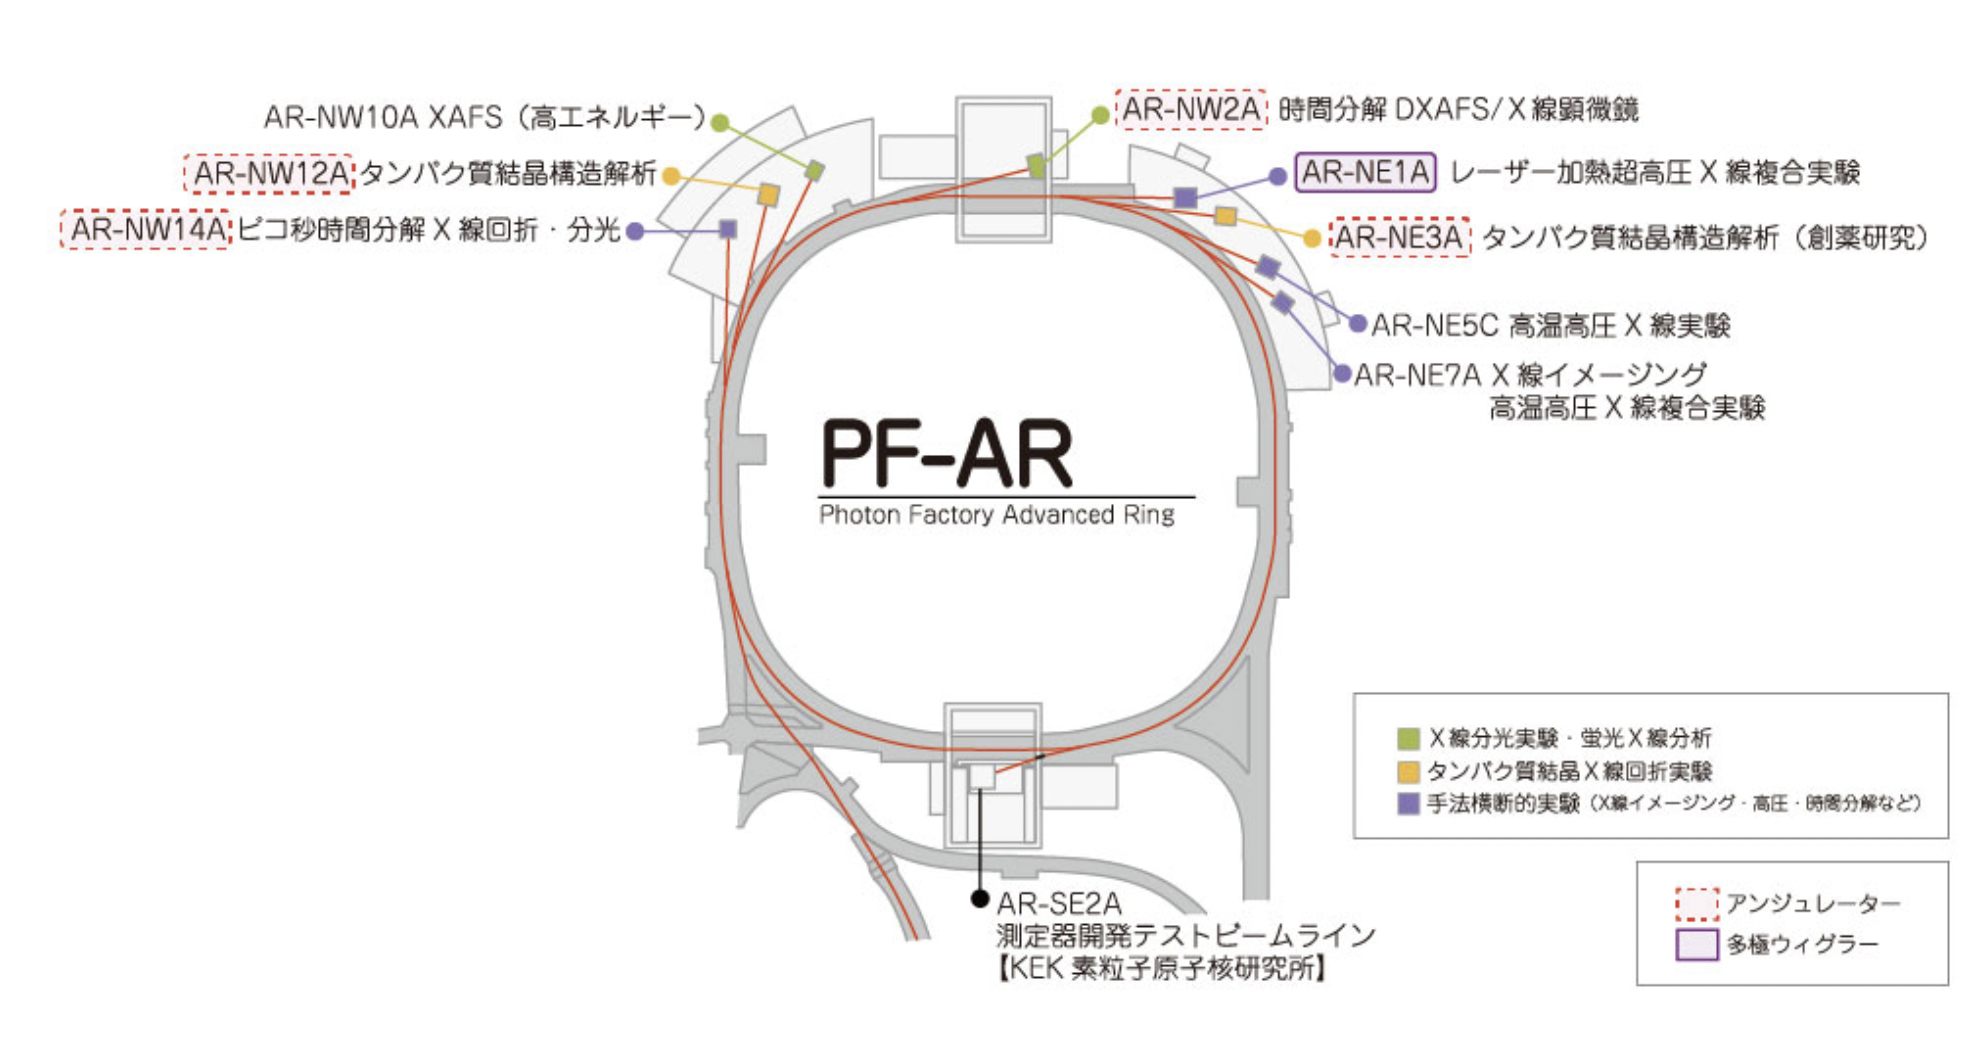
\includegraphics[width=300pt]{./Figure/EBESAnalysis/PFAR.png}
		\caption[PF-ARの概形]{PF-ARの概形。}
		\label{PF-AR}
	\end{center}
\end{figure}


このビームラインは$\SI{6.5}{GeV}$の電子ビームが周回しており、円軌道を荷電粒子が曲がる時に生じる放射光を利用することが可能となる。一方、AR-TBではアドバンスドリングを周回する電子ビームをワイヤー標的へと照射し、生じたガンマ線がコンバータによって電子陽電子対へと変換されることで、電子ビームを取り出している。目的とする運動量の電子ビームを得るために双極電磁石が用いられ、利用可能なエネルギーは$\SI{0.5}{GeV}$-$\SI{5.0}{GeV}$である。

\section{実験セットアップ}
実験セットアップを上から見た模式図を図\ref{calib_setup}に示す。
\begin{figure}[h]
	\begin{center}
		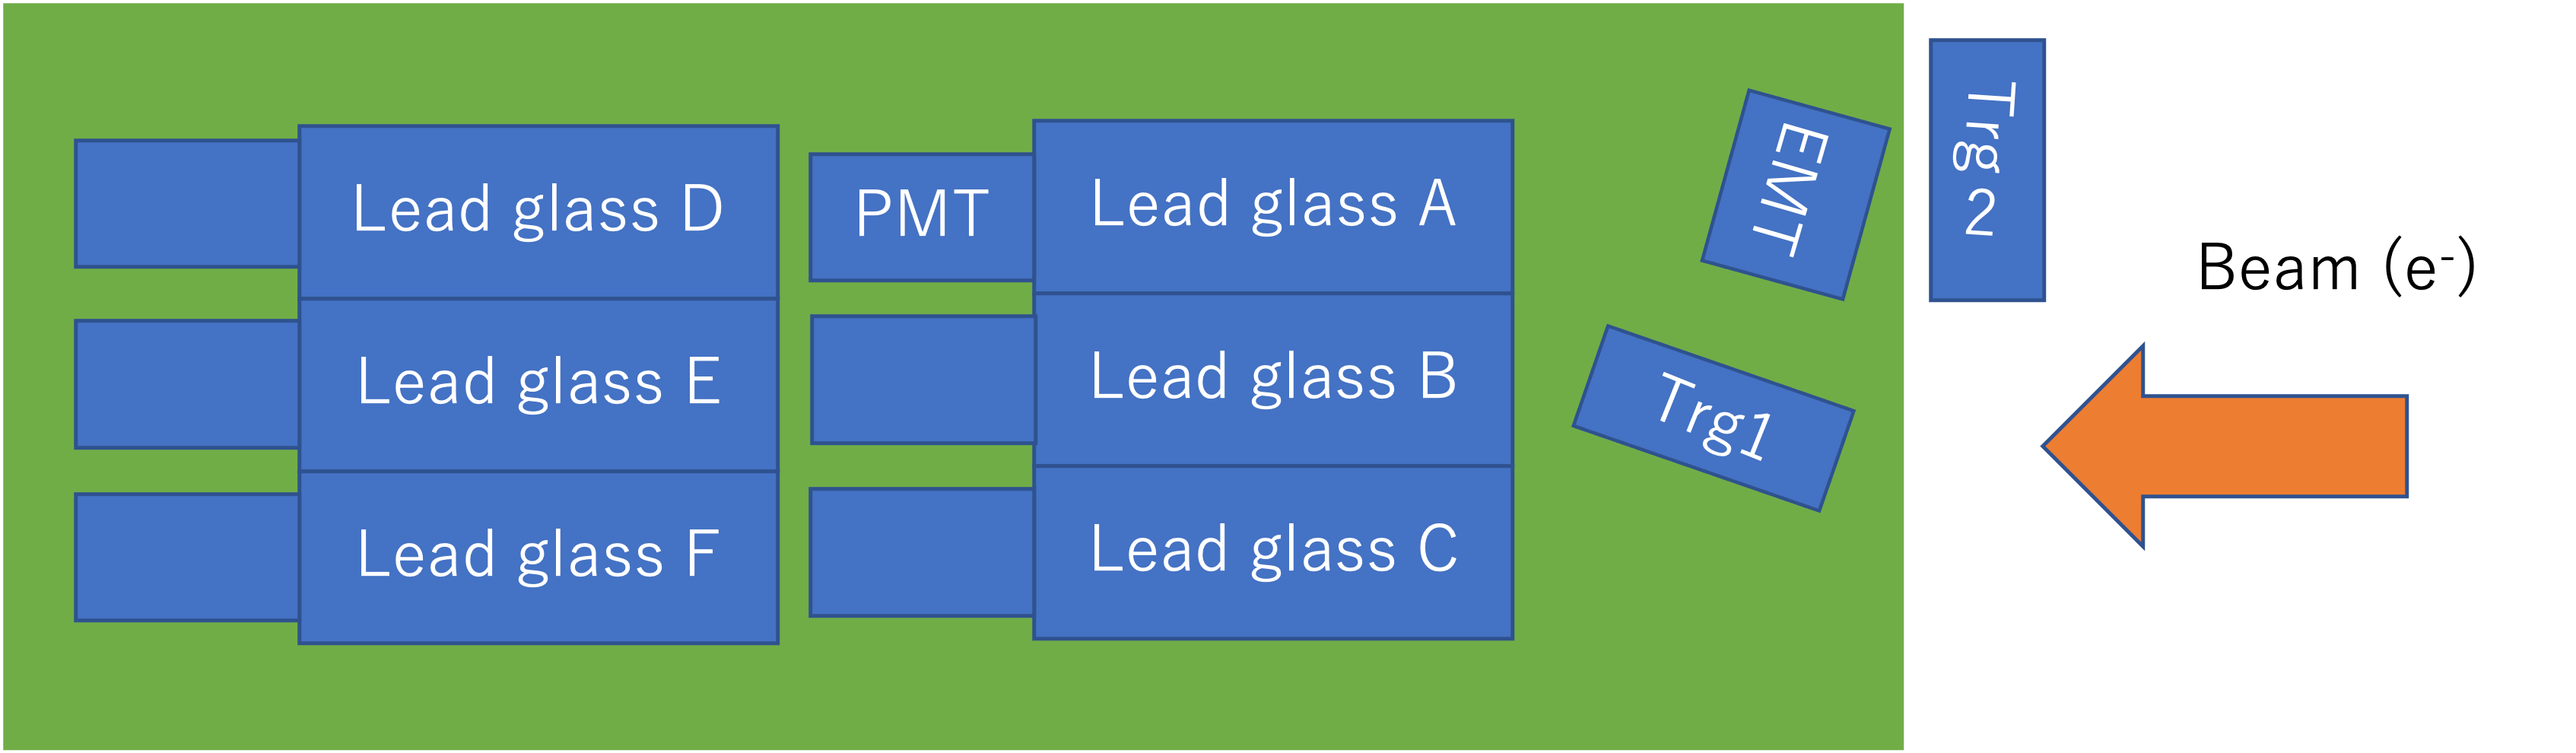
\includegraphics[width=300pt]{./Figure/EBESAnalysis/CalibSetup.png}
		\caption[セットアップの概形]{セットアップの概形。}
		\label{calib_setup}
	\end{center}
\end{figure}


およそ$\SI{1.2}{m}$のステージの上に6つの鉛ガラス検出器を設置し、高電圧電源(High Voltage, HV)と接続した。電子ビームは図右側から入射し、検出器Bに入射する。周囲の検出器はエネルギー漏れを検出するために設置している。トリガーとしてシンチレータを検出器Bの前に設置し、ビームの照射位置を鉛ガラスの中心付近に限定するため角度をつけて配置した。以後これをトリガー1とする。今回、名古屋大学のBelle IIグループと共同で研究を行ったため、検出器AとBの間に電子増倍管(Electron multiplier tube, EMT)およびそのトリガー用のシンチレータが置かれている。このトリガーはトリガー2と呼ぶ。鉛ガラス検出器の信号線はビームライン隣の側室に備えられたNIM(Nuclear Instruments Module)モジュールへと接続され、図\ref{NIM}のように論理回路を組んだ。最終的に信号はCAMAC(Computer Automated Measurement and Control)へと送られ、PCで解析を行った。
\begin{figure}[H]
	\begin{center}
		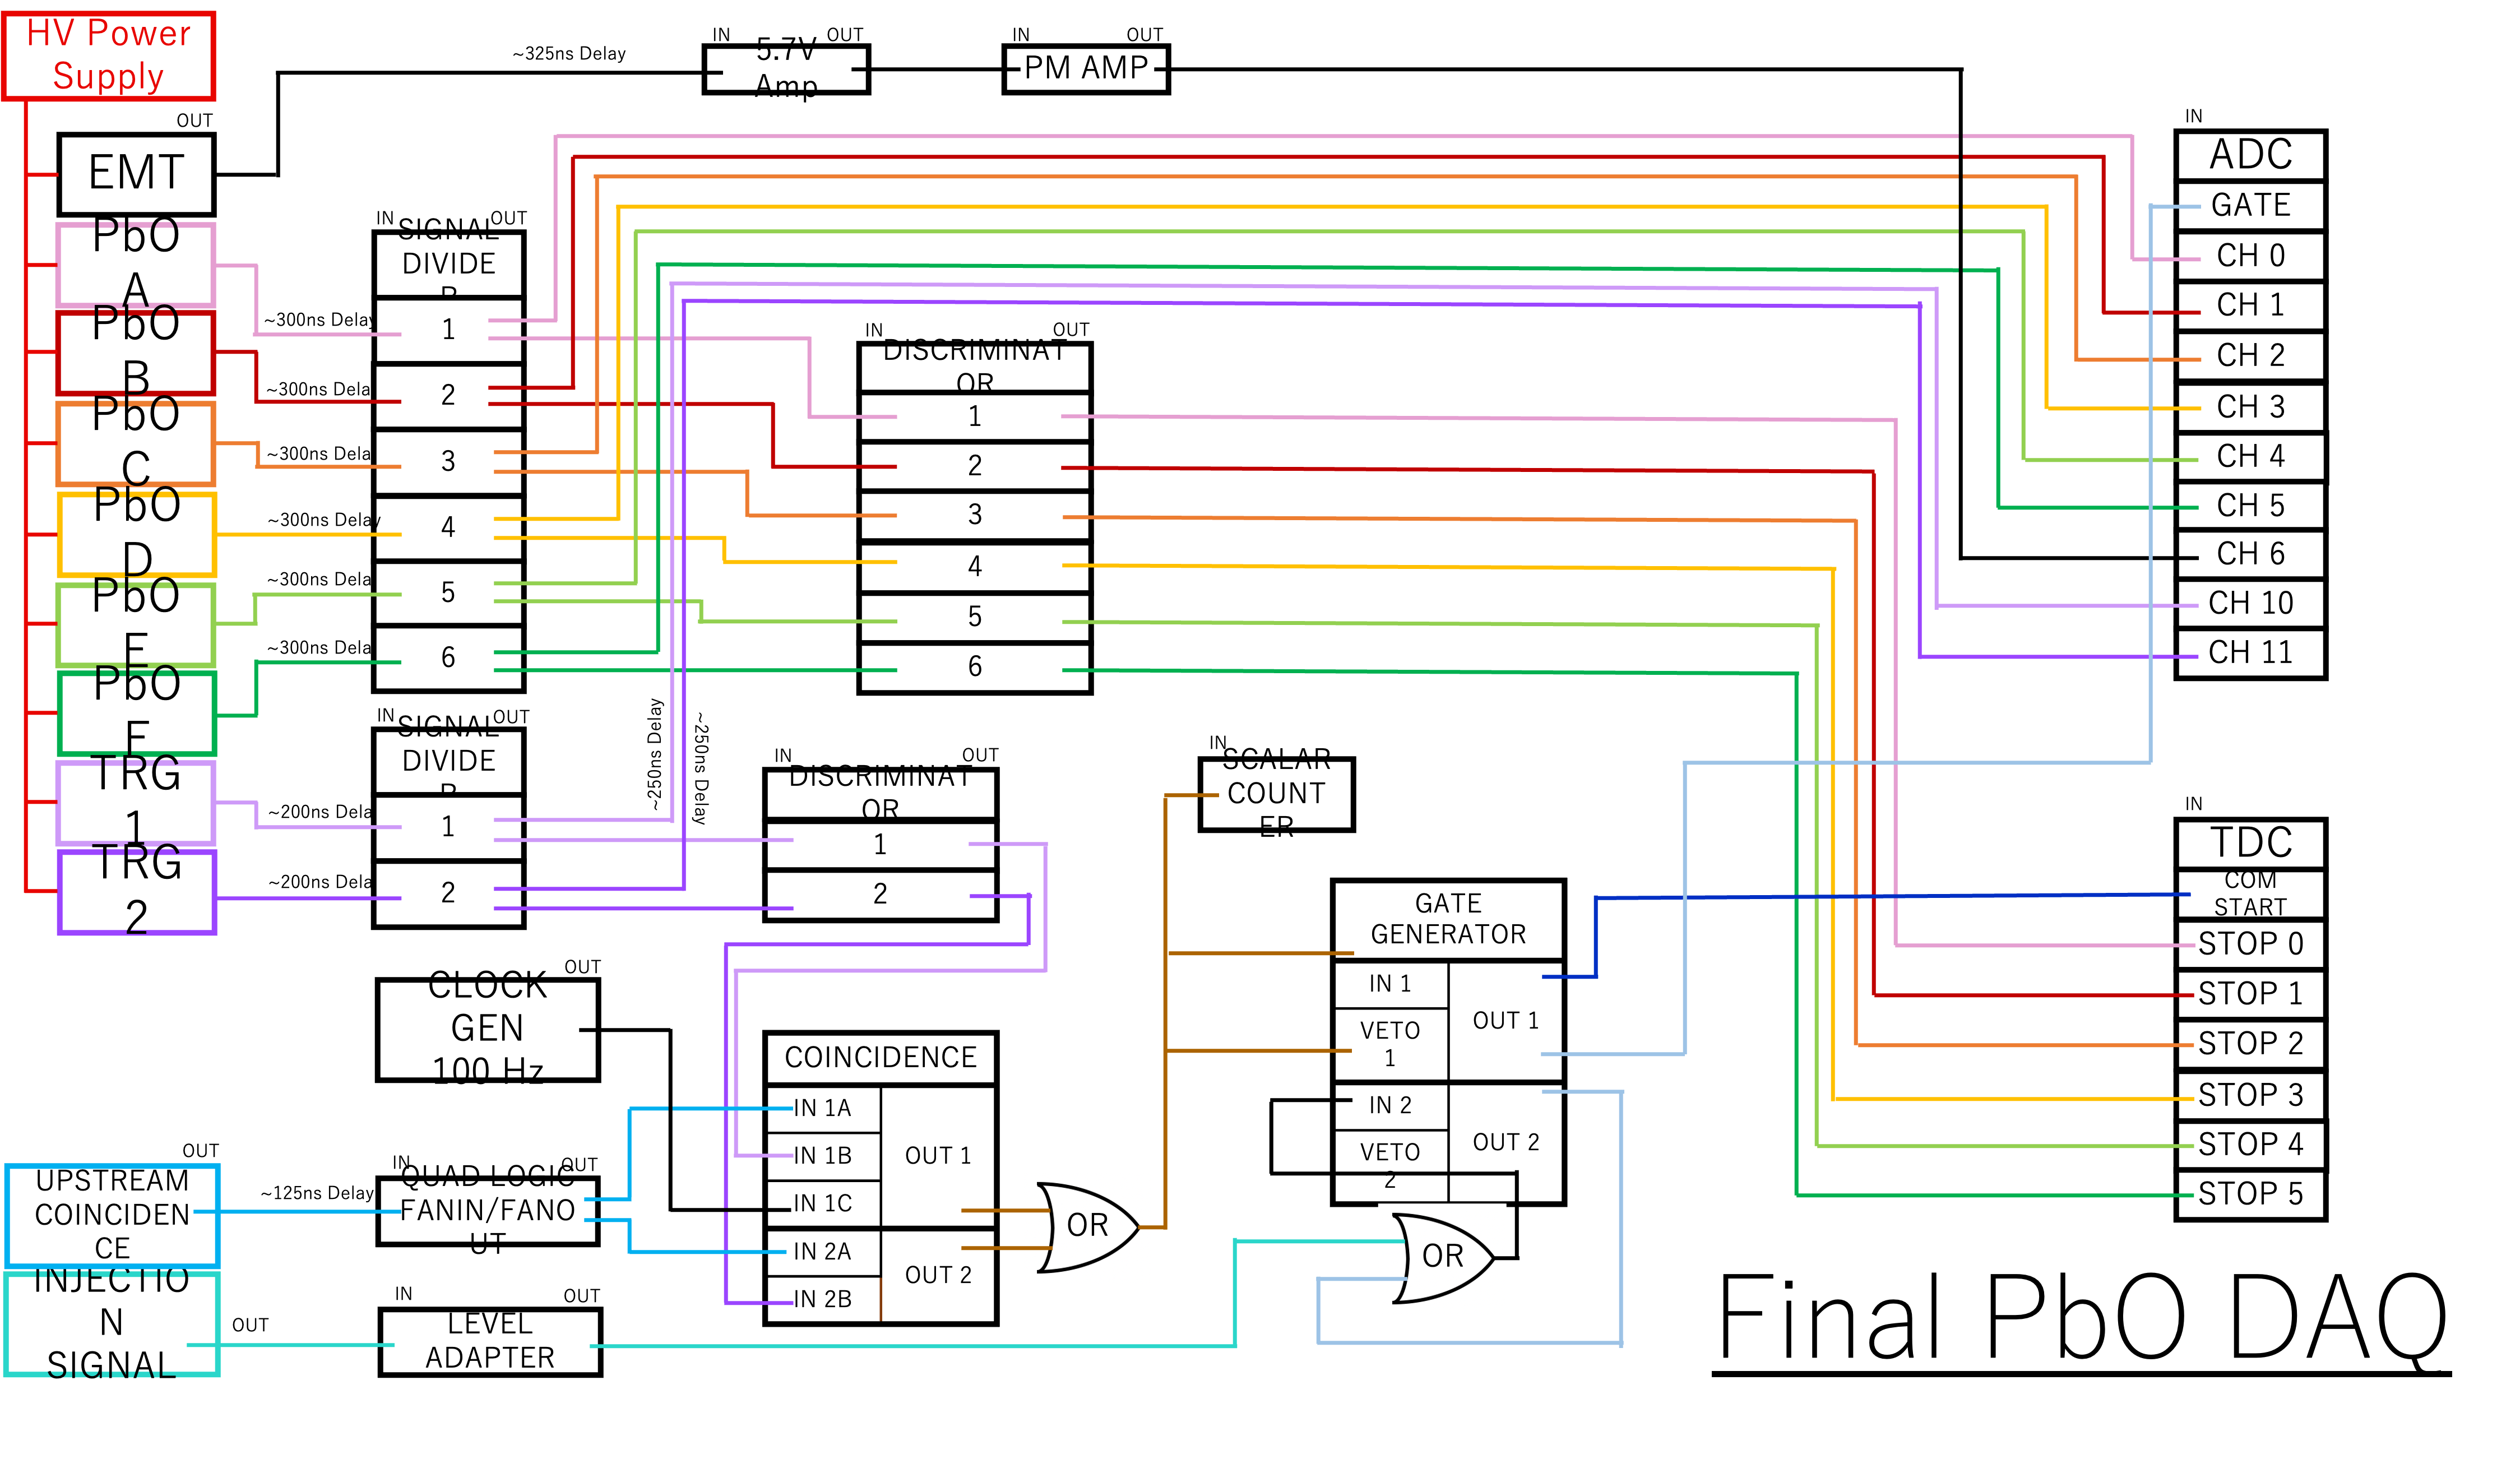
\includegraphics[width=300pt]{./Figure/EBESAnalysis/NIM.png}
		\caption[論理回路の模式図。]{論理回路の模式図。}
		\label{NIM}
	\end{center}
\end{figure}

今回測定のために25個の鉛ガラス検出器を搬入し、全てに対してビーム照射試験を行った。実験は2022年11月17日から21日にかけて行われた。それぞれの検出器に対してまずNIMモジュールから生成したクロック信号をトリガーとしてぺデスタル測定を行った後、トリガーをシンチレータの信号へと変更してビームによる測定へと切り替えた。これをビームのエネルギーを$4.0$、$3.0$、$2.0$、$1.0$、$\SI{0.5}{GeV}$へと変更して繰り返し実行した。ぺデスタル測定とビーム測定の合間に検出器Bの信号線をオシロスコープへと接続し、電圧値が$\SI{200}{mV}$となるように検出器のHVを調節した。

トリガーレートはビームのエネルギーごとに異なっており、トリガー1を用いて図\ref{TrgRate}のように測定された。これは\SI{60}{s}当たりに測定された平均回数を記録している。

\begin{figure}[H]
	\begin{center}
		\includegraphics[width=200pt]{./Figure/EBESAnalysis/trg_rate_reduce.pdf}
		\caption[トリガーレート]{トリガー1の1秒当たりのトリガーレート。\SI{60}{s}当たりに測定された平均回数を記録している。}
		\label{TrgRate}
	\end{center}
\end{figure}

\section{データに対する補正}
測定されたデータを解析するにあたり、いくつかの補正を行った。まず、ペデスタルはビームが検出器に入射していない場合でも生じるADCのベースラインであり、その幅は検出器ノイズに依存する。今回はソフトウェア上で減算した。ペデスタル測定において得られたデータをガウシアン関数
\begin{equation}
f(x) = p_0\exp\left(-\frac{(x-p_1)^2}{2p_2^2}\right)
\end{equation}
(ただし、$p_0$、$p_1$、$p_2$は定数。)でフィットし、その平均値$p_1$を直後に測定したビーム測定の結果から減算した。さらに、ビームが検出器Bに入射したタイミングのデータのみを抽出するためにトリガーのデータのうち、ペデスタルを減算したADCが250以上550以下となるイベントをセレクションした。それぞれのプロットを図\ref{Pedestal}、\ref{TrgSelection}、\ref{CorrectBeam}に示す。
\begin{figure}[H]
	\begin{center}
		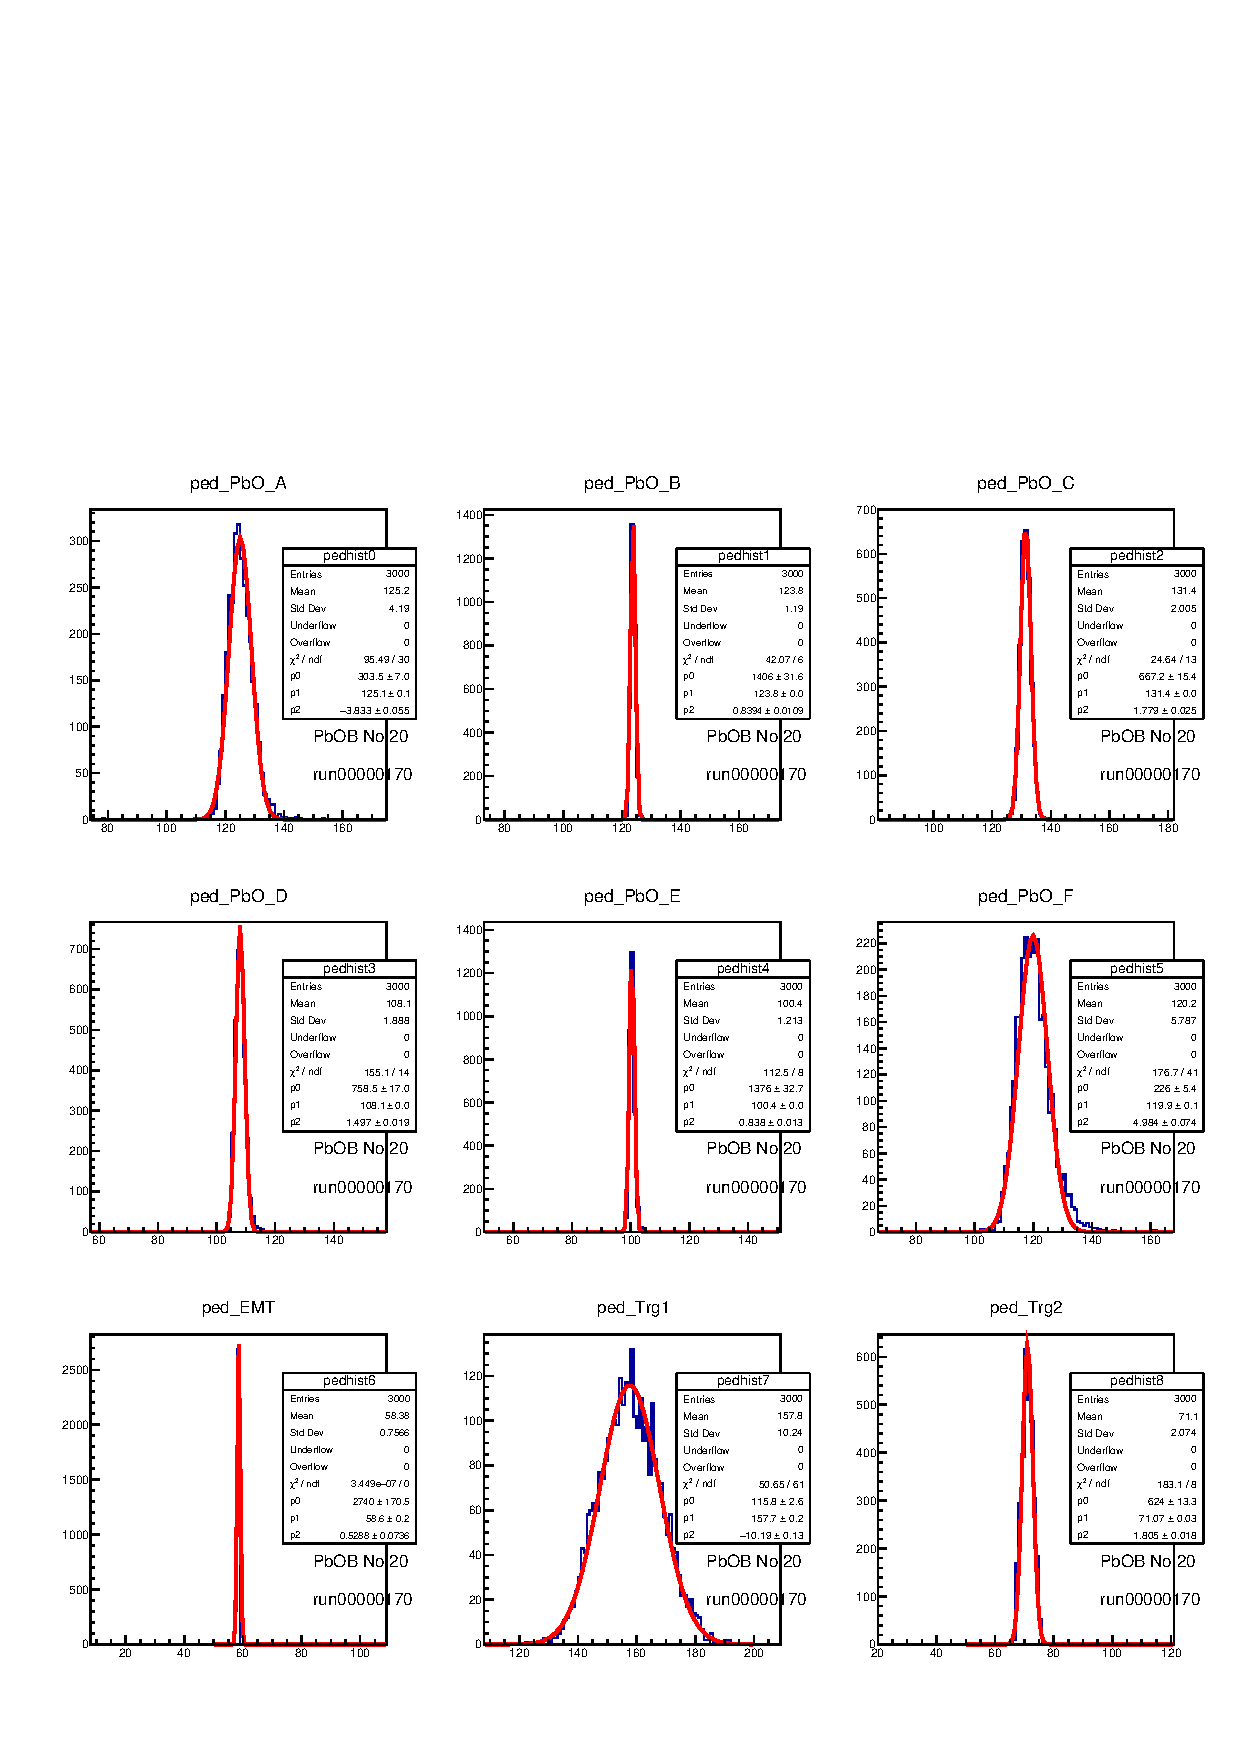
\includegraphics[width=200pt]{./Figure/EBESAnalysis/Pedestal.pdf}
		\caption[ペデスタルデータの一例]{ペデスタルデータを表すヒストグラムの一例。それぞれPbOAからPbOFおよびトリガー1、トリガー2、EMTを表している。横軸は各検出器から出力されたADCであり、縦軸はカウント数を示す。PbOBの後の数字は鉛ガラス検出器の整理番号を示す。}
		\label{Pedestal}
	\end{center}
\end{figure}

\begin{figure}[H]
	\begin{center}
		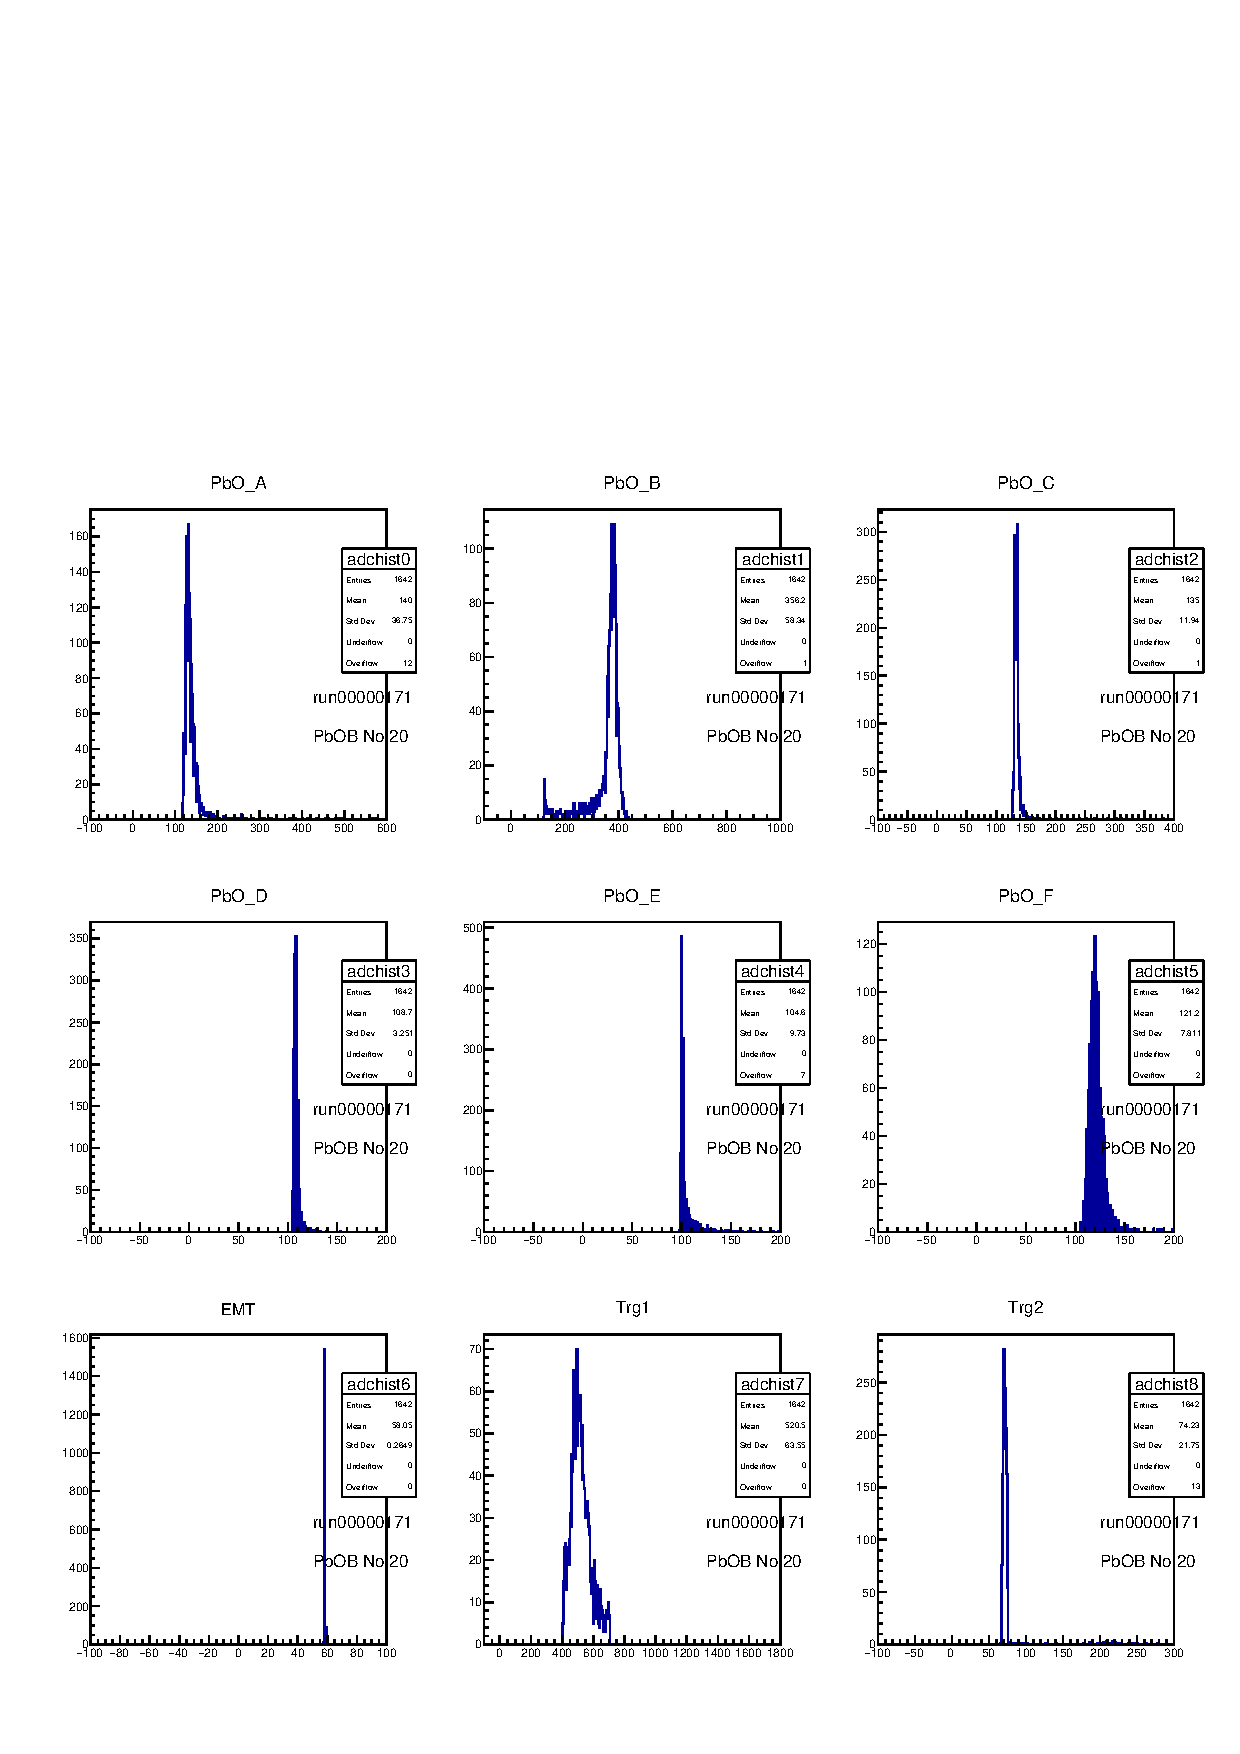
\includegraphics[width=200pt]{./Figure/EBESAnalysis/TrgSelection.pdf}
		\caption[トリガーによりイベント選別をおこなった後の各検出器の応答]{トリガー1によりイベント選別をおこなった後の各検出器の応答。横軸は各検出器から出力されたADCであり、縦軸はカウント数を示す。トリガー1のADCが250から550までのイベントを選別している。}
		\label{TrgSelection}
	\end{center}
\end{figure}

\begin{figure}[H]
	\begin{center}
		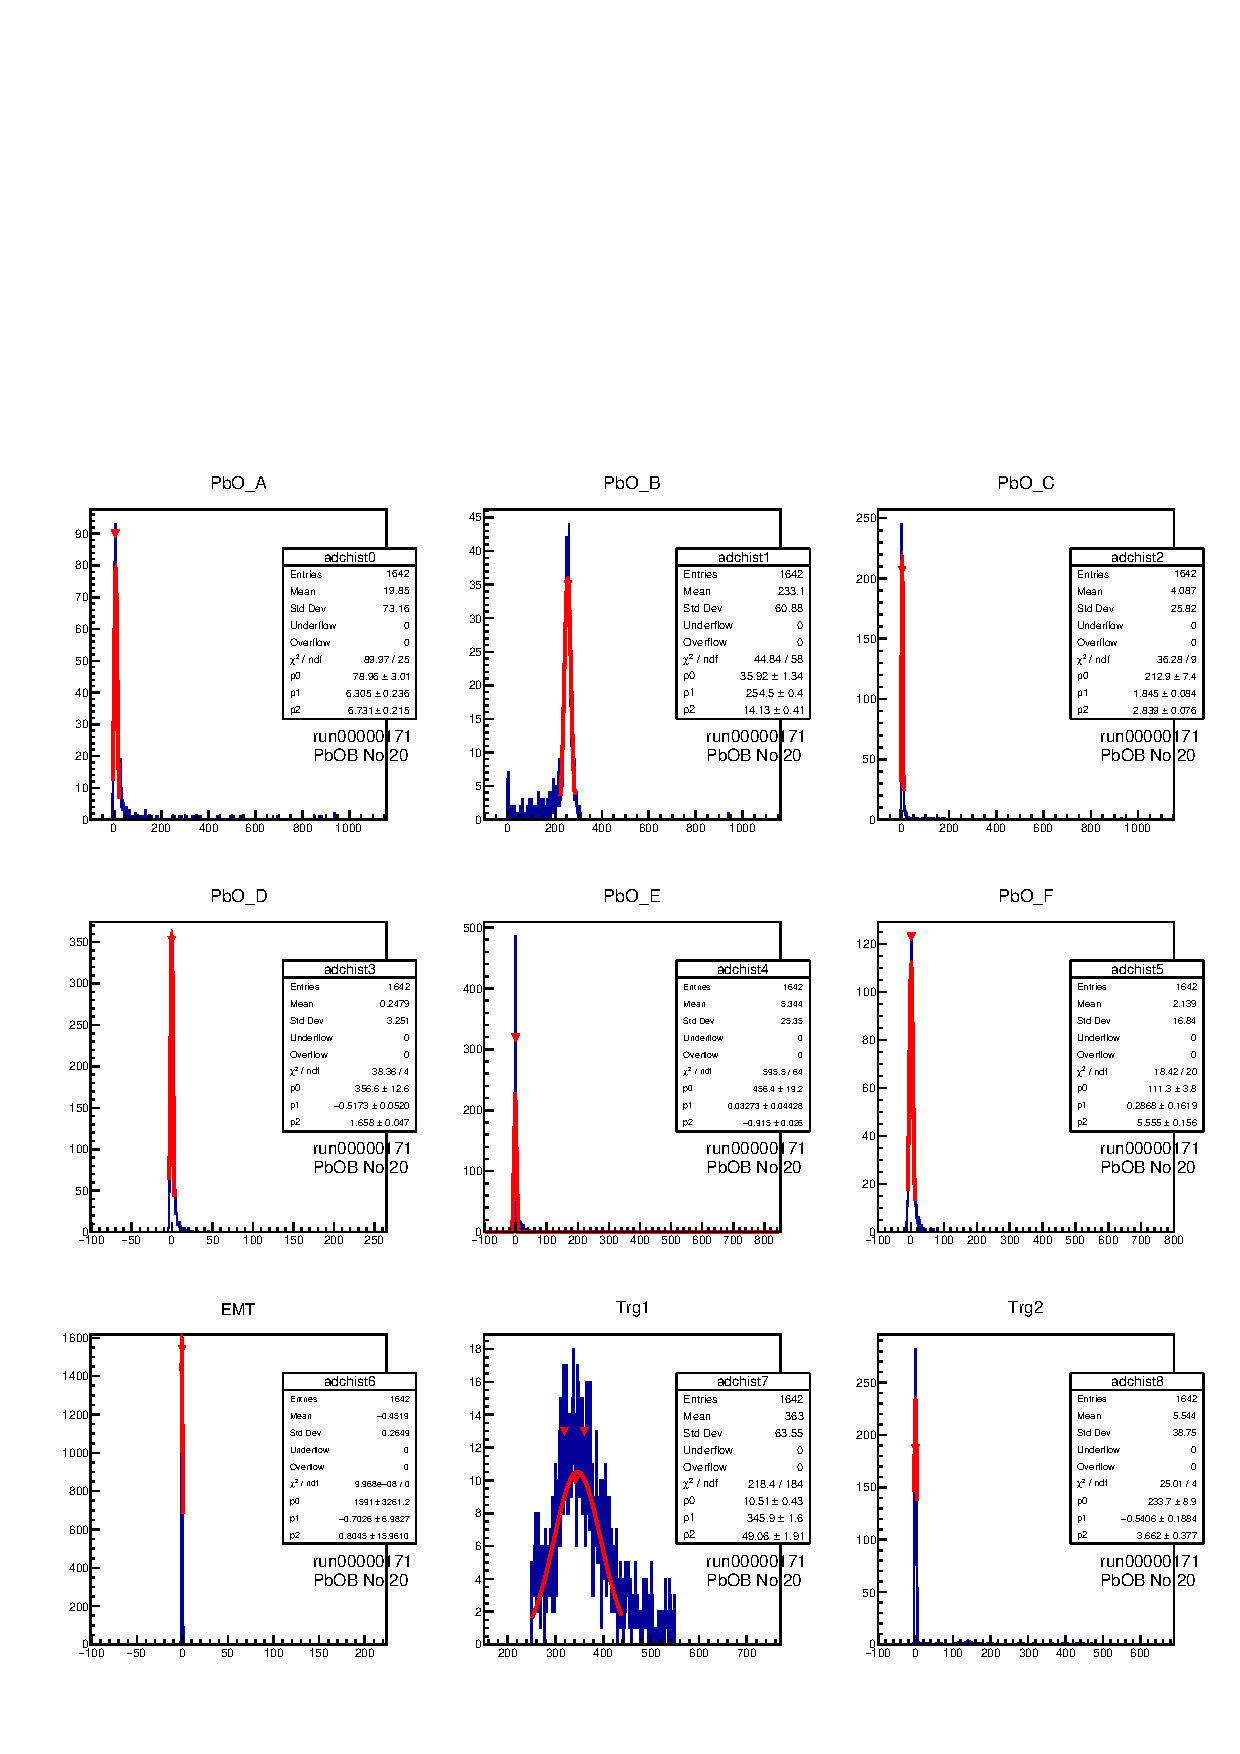
\includegraphics[width=200pt]{./Figure/EBESAnalysis/CorrectBeam.pdf}
		\caption[トリガーによるイベント選別とペデスタル減算により補正した後のデータ]{トリガーによるイベント選別とペデスタル減算により補正した後のデータ。ペデスタルデータは直前に測定したものを用いた。横軸は各検出器から出力されたADCであり、縦軸はカウント数を示す。}
		\label{CorrectBeam}
	\end{center}
\end{figure}

\section{エネルギー較正}
ペデスタルデータを減算した検出器Bのデータに対して、ガウシアンフィットを行い、その中央値を各検出器ごとにビームエネルギーに対してプロットすることでエネルギー較正を行った。その結果を一部の検出器について図\ref{calib}に示す。ALPsの生成によって検出器に生じる信号は今回測定を行った領域と重なり、線形性を保っていることが望ましい。各点を1次関数
\begin{equation}
y = p_0x+p_1
\end{equation}
でフィッティングを行った。ただし、$p_0$、$p_1$は定数。この直線と$y$切片を$0$で固定した$y'=p'_0x'$を比較し、フィッティングの結果として得られたパラメータを図\ref{calib_para}に示した。この結果から、データの線形性は保てているものの$y$切片に各検出器で一様なズレが生じており、$y$切片が全ての検出器で負となっていることがわかる。

\begin{figure}[H]
	\begin{center}
		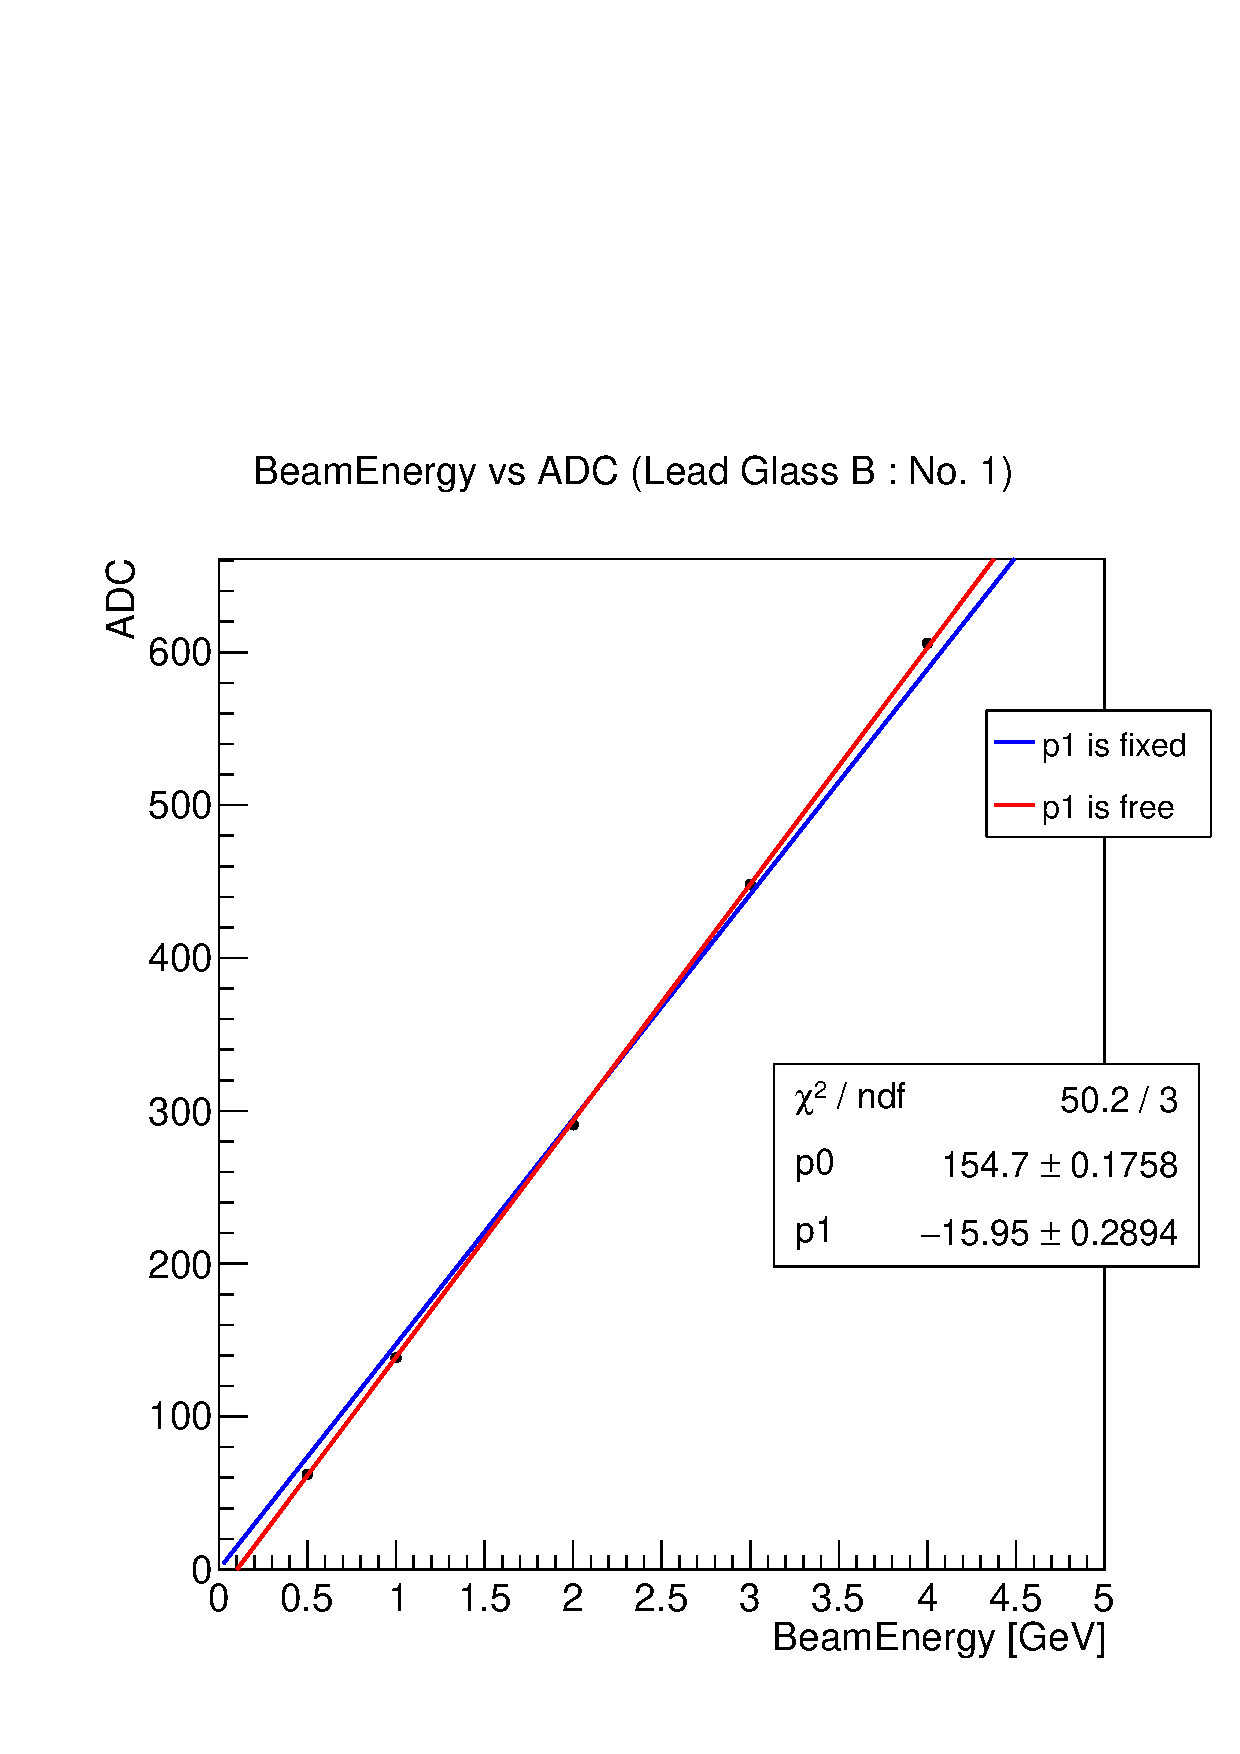
\includegraphics[width=200pt]{./Figure/EBESAnalysis/calib.pdf}
		\caption[ビームエネルギーとADCの相関]{ビームエネルギーとADCの相関。赤線はデータを式(6.2)でフィッティングしたもの。青線は$y$切片を0で固定したもの。}
		\label{calib}
	\end{center}
\end{figure}

\begin{figure}[H]
	\begin{subfigure}{.5\textwidth}
		\begin{center}
 		 	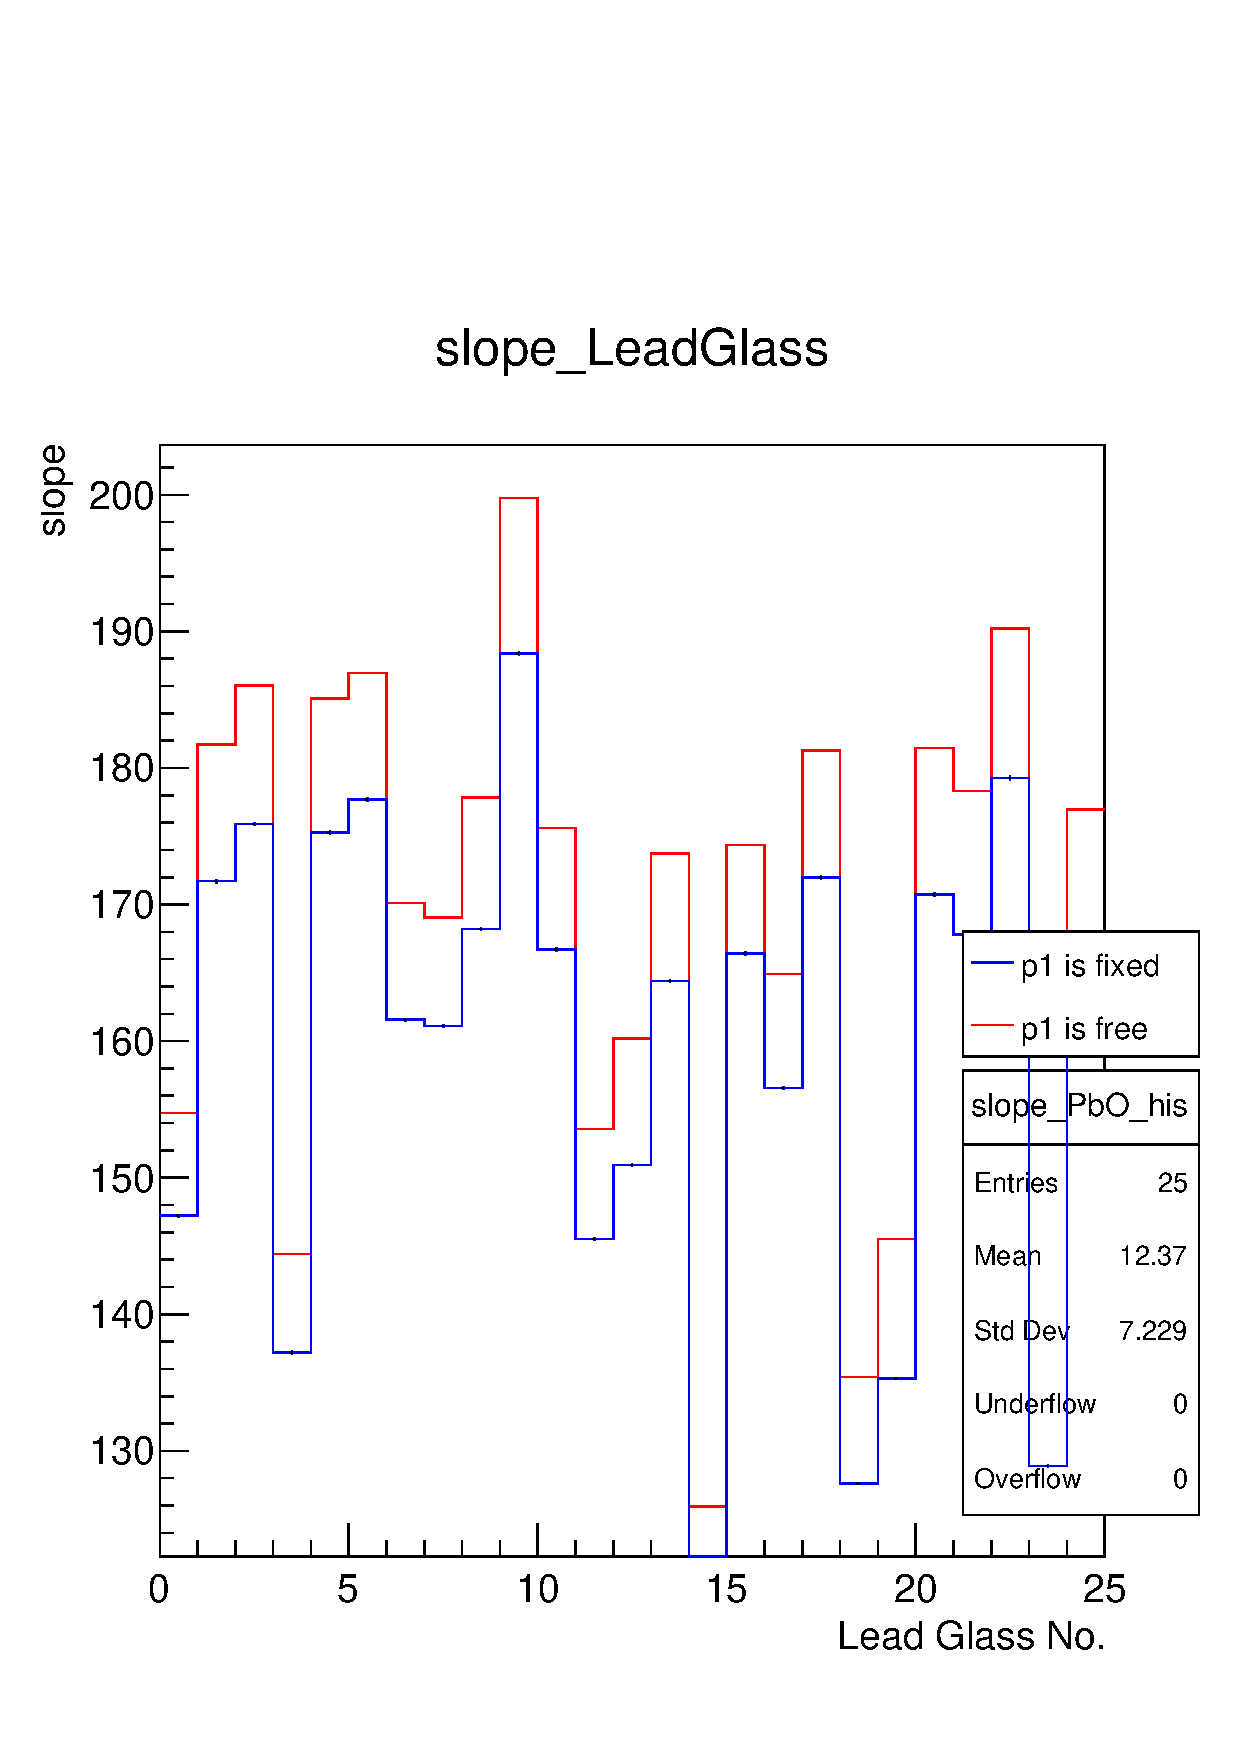
\includegraphics[width=200pt]{./Figure/EBESAnalysis/calibration_slope_fix.pdf} 
			  \caption{各検出器のフィッティングパラメーター $p_0$および$p'_0$}
  			\label{fig:sfig1}
 		\end{center}
	\end{subfigure}
	\begin{subfigure}{.5\textwidth}
		\begin{center}
			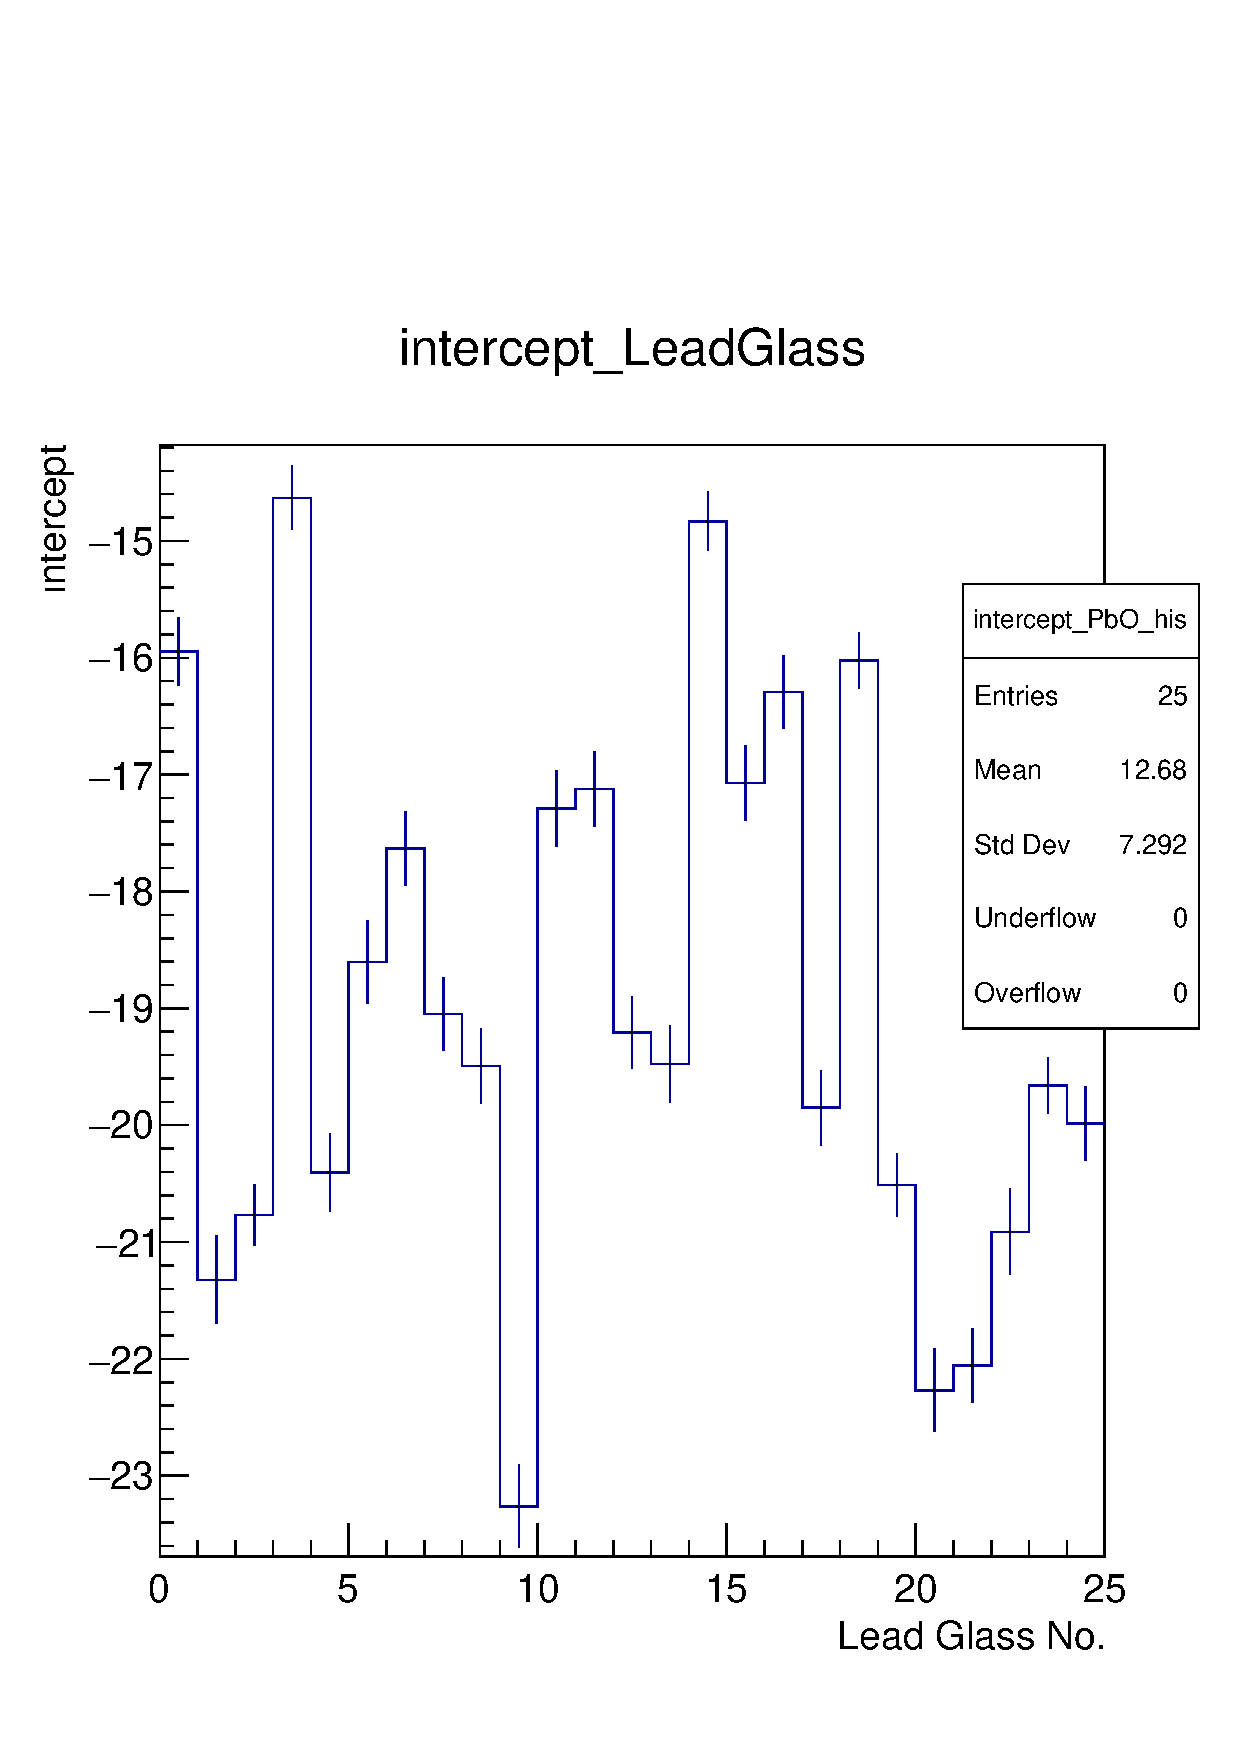
\includegraphics[width=200pt]{./Figure/EBESAnalysis/calibration_intercept.pdf}%.5\linewidth]{./Figure/DLAnalysis/Input2.png}
			\caption{各検出器のフィッティングパラメーター $p_1$}
			\label{fig:sfig2}
		\end{center}
	\end{subfigure}
	\caption[フィッティングパラメーターの比較]{各検出器のフィッティングパラメータの比較。(a)は$p_0$および$p_0'$を、(b)は$p_1$をプロットしている。また、グラフ(a)で青い線はbを0に固定した場合のヒストグラムを、赤い線はフリーにしたものを示している。}
	\label{calib_para}
\end{figure}

ズレの影響とビームエネルギーに依存性があるかどうかを調べるために、フィッティング関数の$x$切片を調べた。図\ref{inter_x}に各検出器の$x$切片をプロットする。
\begin{figure}[H]
	\begin{center}
		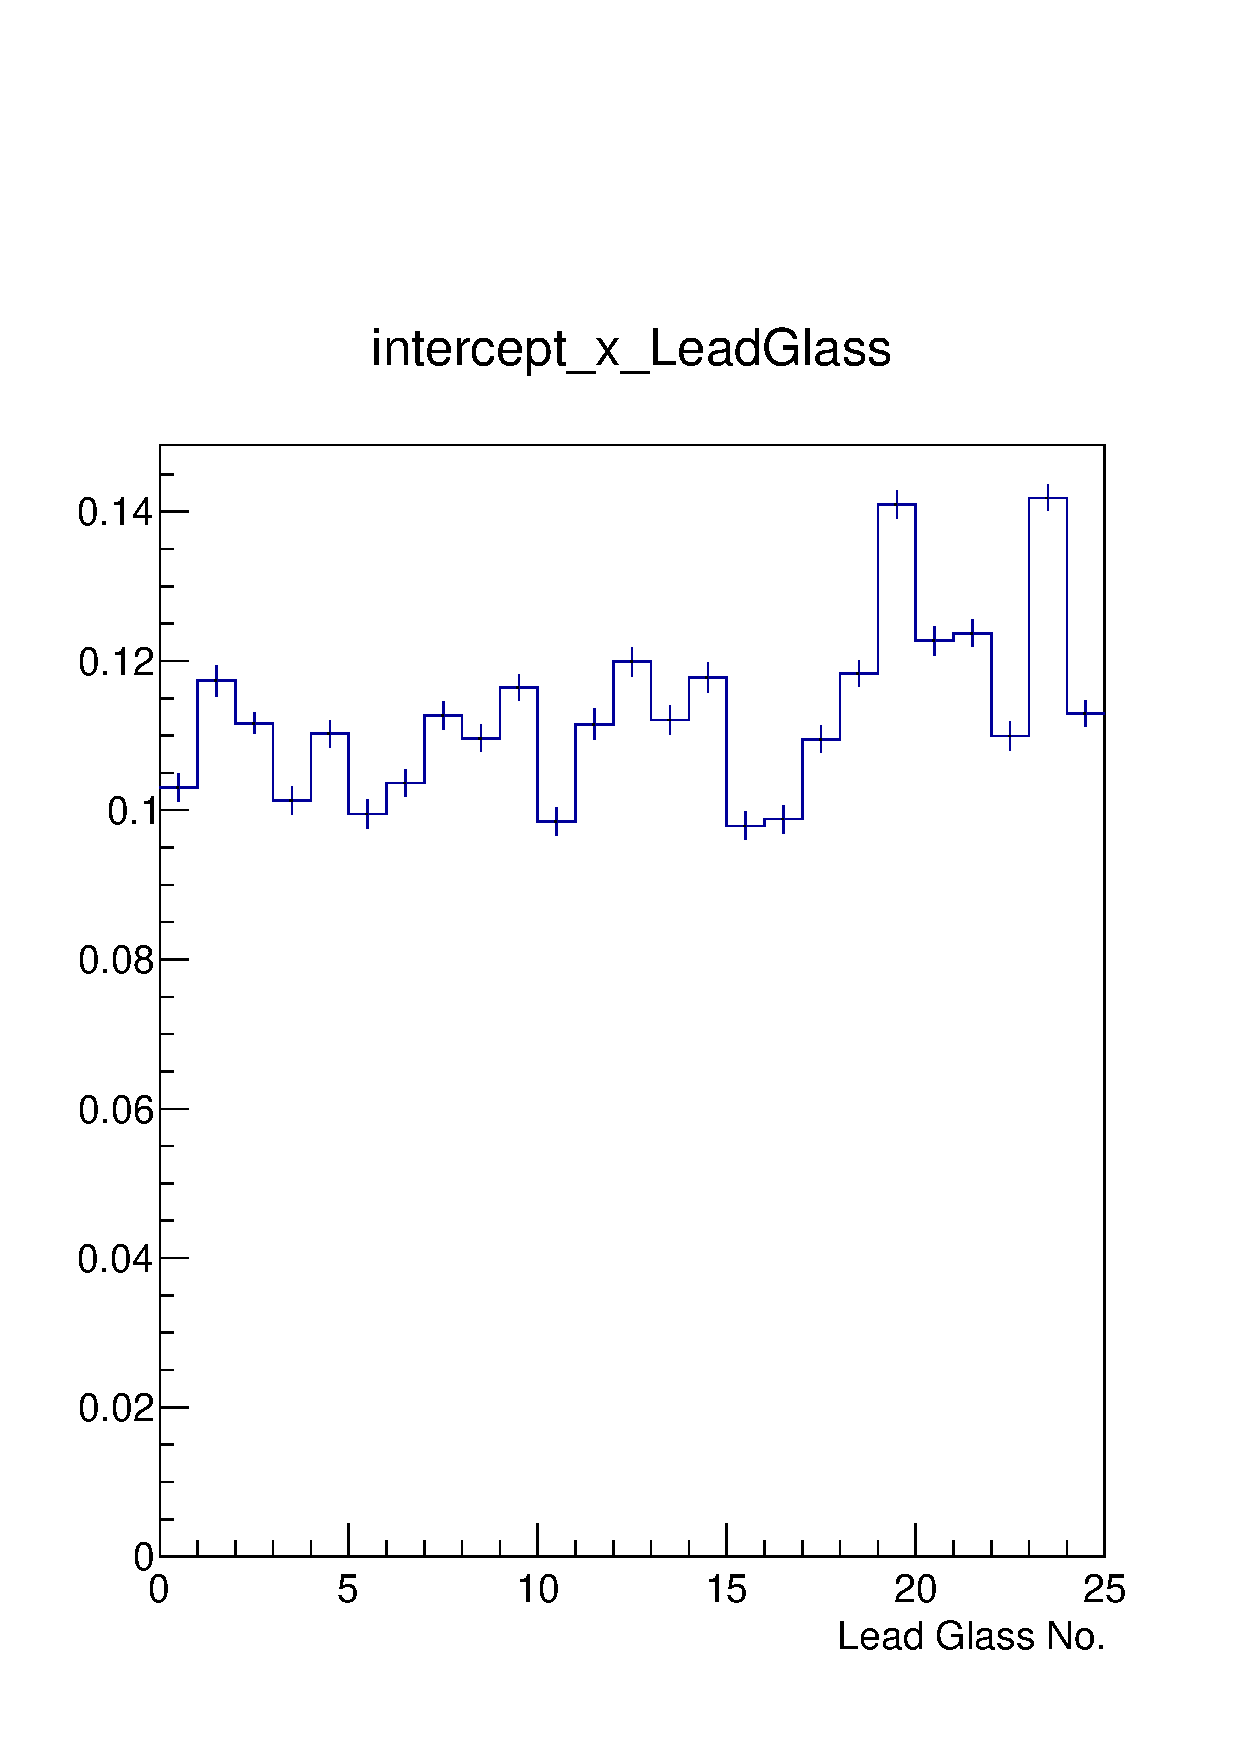
\includegraphics[width=200pt]{./Figure/EBESAnalysis/calibration_intercept_x.pdf}
		\caption[フィッティング関数の$x$切片]{フィッティング関数の$x$切片。}
		\label{inter_x}
	\end{center}
\end{figure}

$x$切片が各検出器で同程度となっており、検出器ではなくビームエネルギーによって較正直線がずれていることが示唆される。

これらの$x$切片の平均値を計算すると、$0.1128\pm\SI{0.0018}{GeV}$となり、この値をビームエネルギーから減算して再度プロットした。その結果を図\ref{calib_re}に示す。
\begin{figure}[h]
	\begin{center}
		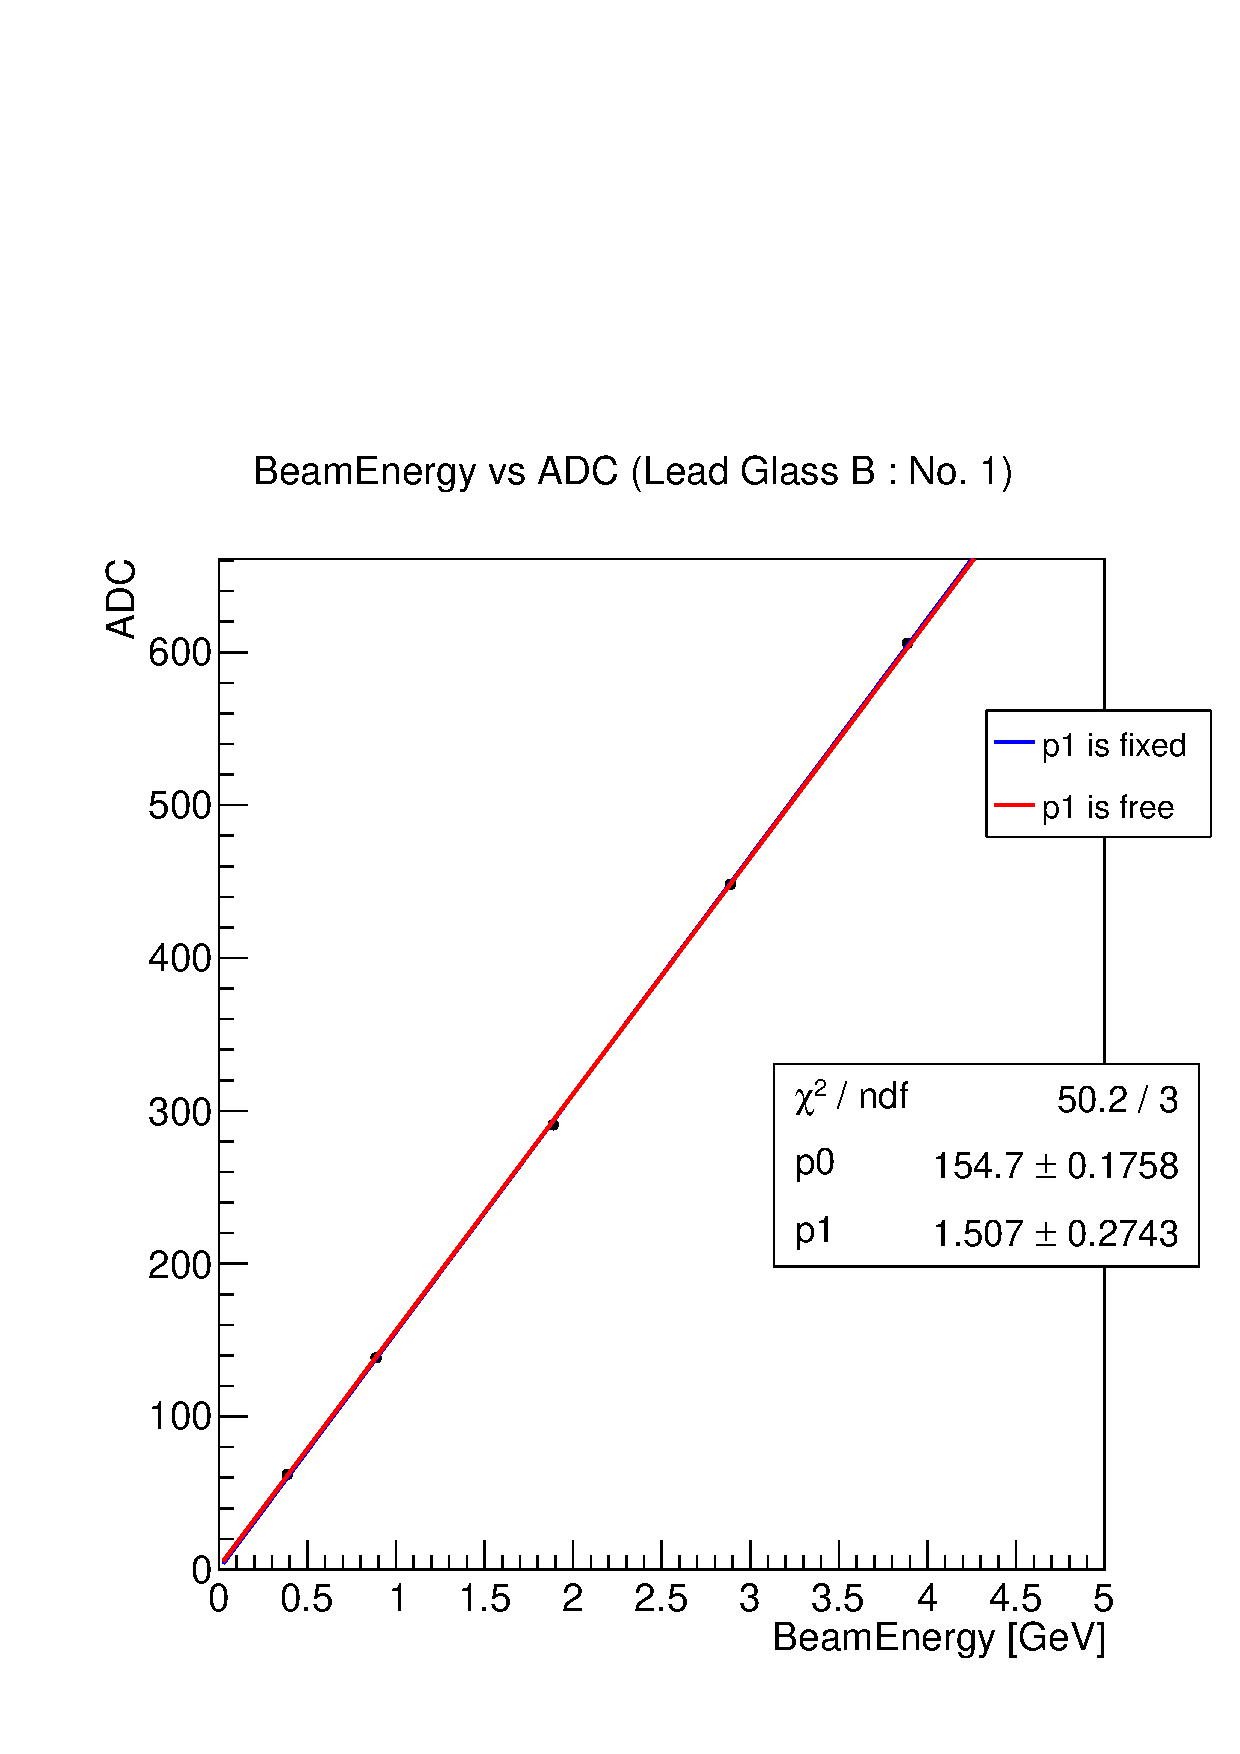
\includegraphics[width=200pt]{./Figure/EBESAnalysis/calibration_re.pdf}
		\caption[ビームエネルギー補正後のフィッティング]{ビームエネルギー補正後のフィッティング。}
		\label{calib_re}
	\end{center}
\end{figure}

この図を見ると、十分な線形性が得られていることが分かる。本実験で使用したビームラインは昨年度に新設されたものであり、エネルギーに不定性が存在する可能性がある。そのため、今後ビームエネルギーの検証が必要である。

%今回、ビームエネルギーの設定はビームラインに備え付けられたオペレーションシステムから行われた。今回の結果からこの設定と実際のビームエネルギーに差がある可能性が示唆される。

\section{エネルギー分解能測定}
検出器Bのデータのガウシアンフィットに対して、ガウシアンの幅をプロットすることでエネルギー分解能の評価を行った。エネルギー分解能$\frac{\sigma}{E}$はビームエネルギーの関数として3つの項をもち、
%%%%%%%%%%%%%%%%%%%%%%%%%%%%%%%%%%%%%%%%%%%%%%%%%%%%%%%%%%%%%%%%%%%%%%%%%%%%%
\begin{comment}
\[
\frac{\sigma}{E} = \frac{p_0}{\sqrt{E}}+p_1+\frac{p_2}{E}
\]
と表される。ここで、$p_0$、$p_1$、$p_2$は定数である。それぞれの項は統計項、定数項、ノイズ項と呼ばれ、この関数でフィッティングを行った。結果を図\ref{res}に示す。なお、本論文中では検出器1に対して行った解析のみ示している。%また、それぞれの検出器のフィッティングパラメータを図に示す。
\begin{figure}[h]
	\begin{center}
		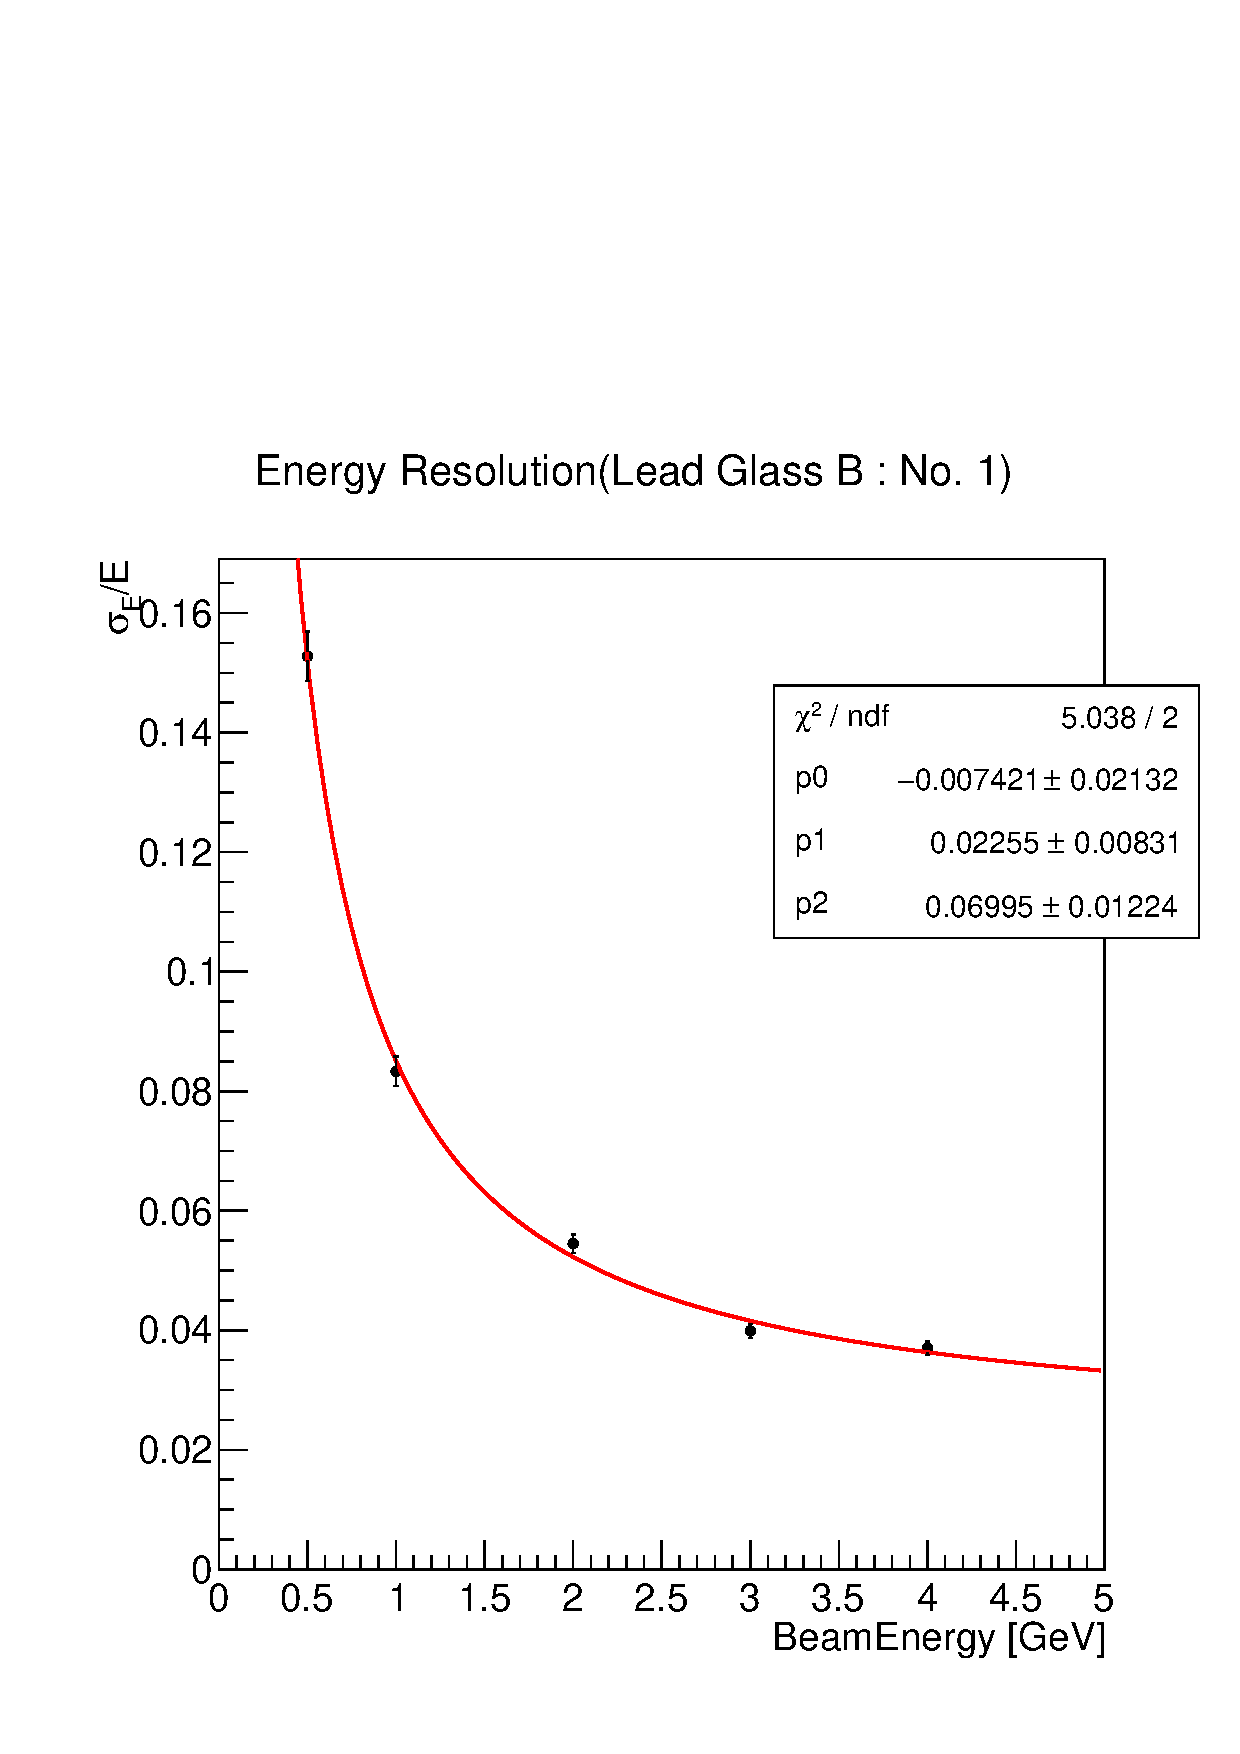
\includegraphics[width=200pt]{./Figure/EBESAnalysis/res.pdf}
		\caption[ビームエネルギー分解能のフィッティング]{ビームエネルギー分解能のフィッティング。}
		\label{res}
	\end{center}
\end{figure}

このフィッティングでは先ほど考慮したビームエネルギーの補正を含んでいない。%この図から、多くの検出器について負の定数項が生じていることがわかる。
この図から、いくつかの点に対してフィッティングが合っておらず、またパラメータ$p_0$が負の値として得られた。
これは、$\SI{4.0}{GeV}$より高エネルギーのデータが足りないために生じていることが原因として考えた。
対策として、フィッティングパラメータを減らすことでフィッティングが改善しないか確かめた。パラメータ$p_0$および$p_1$、パラメータ$p_0$のみでフィッティングを行った結果を\ref{res_twopara}に示す。

\begin{figure}[H]
	\begin{subfigure}{.5\textwidth}
		\begin{center}
 		 	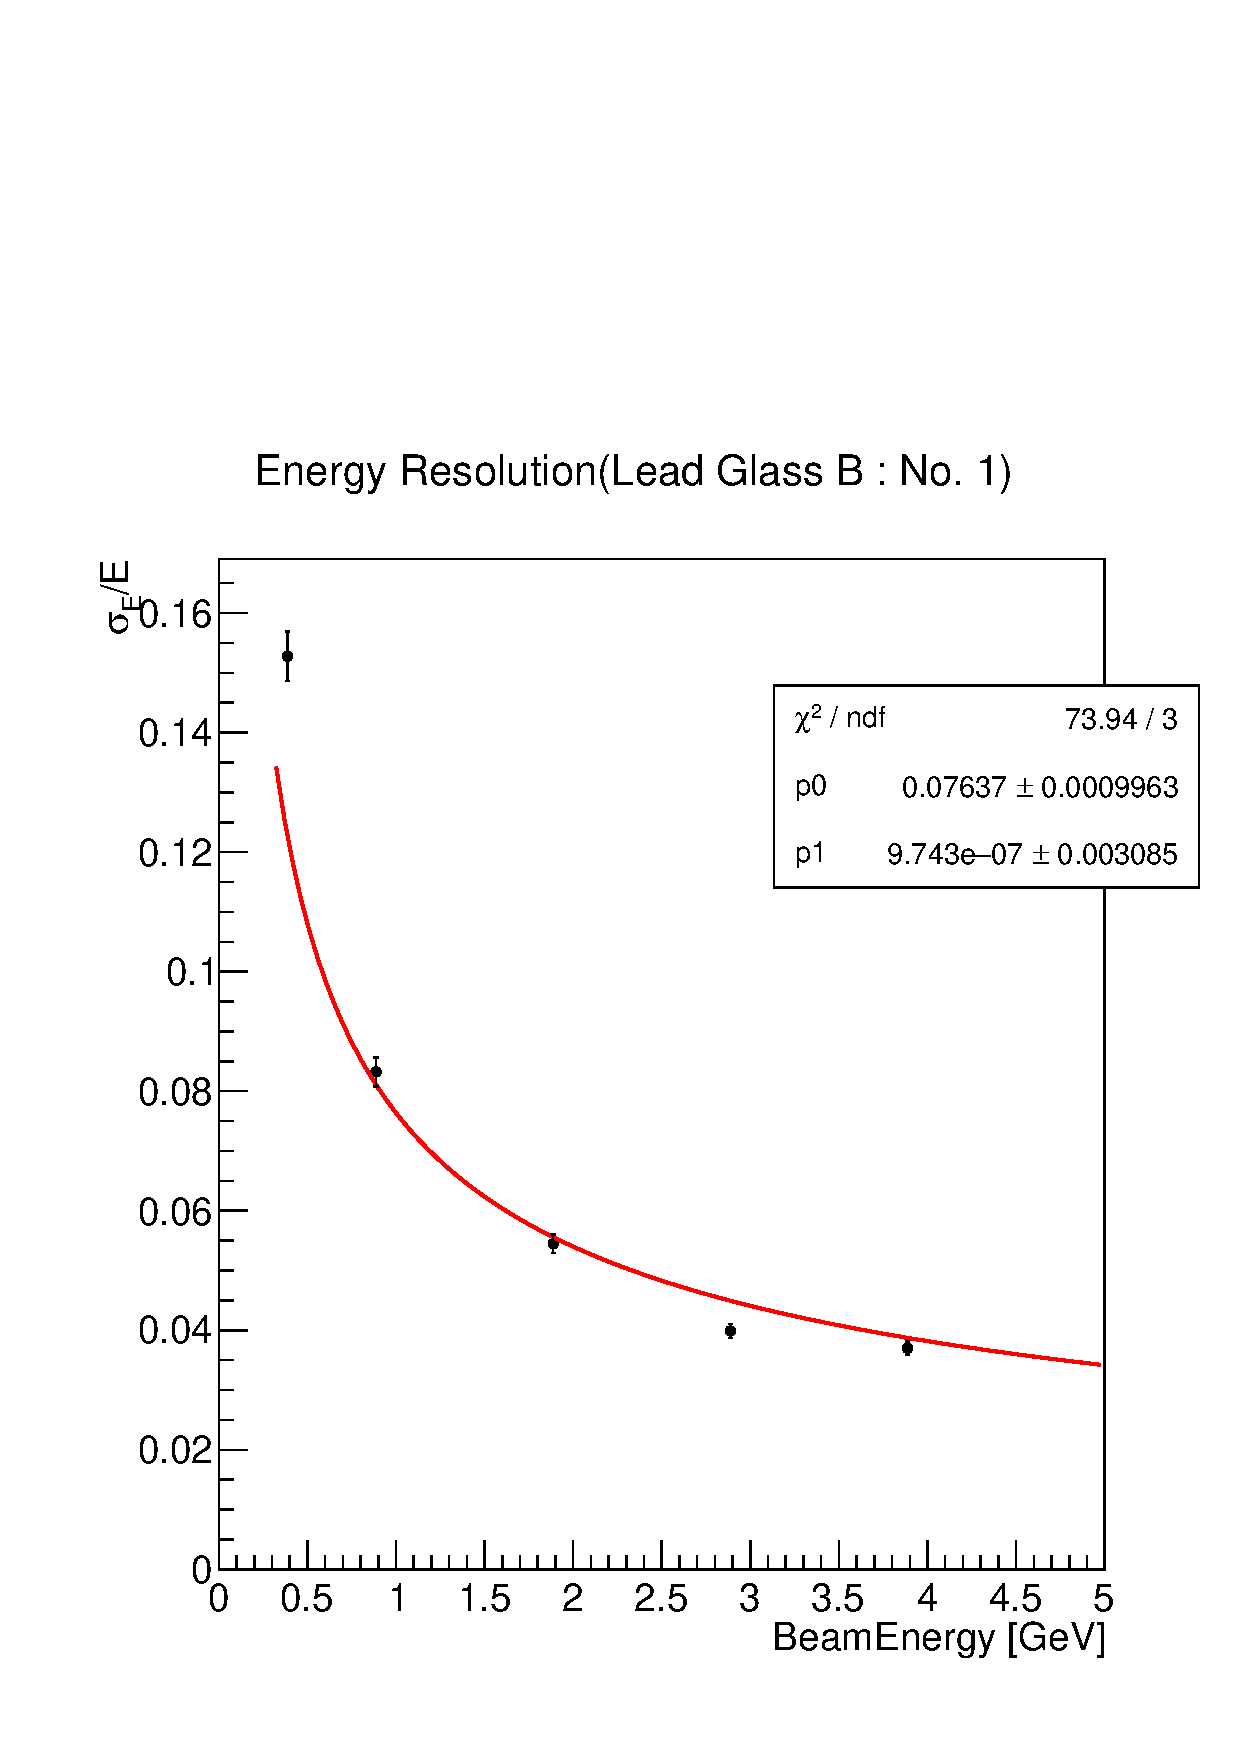
\includegraphics[width=200pt]{./Figure/EBESAnalysis/res_twopara.pdf} 
			  \caption{$p_0$および$p_1$によるフィッティング}
  			\label{fig:sfig1}
 		\end{center}
	\end{subfigure}
	\begin{subfigure}{.5\textwidth}
		\begin{center}
			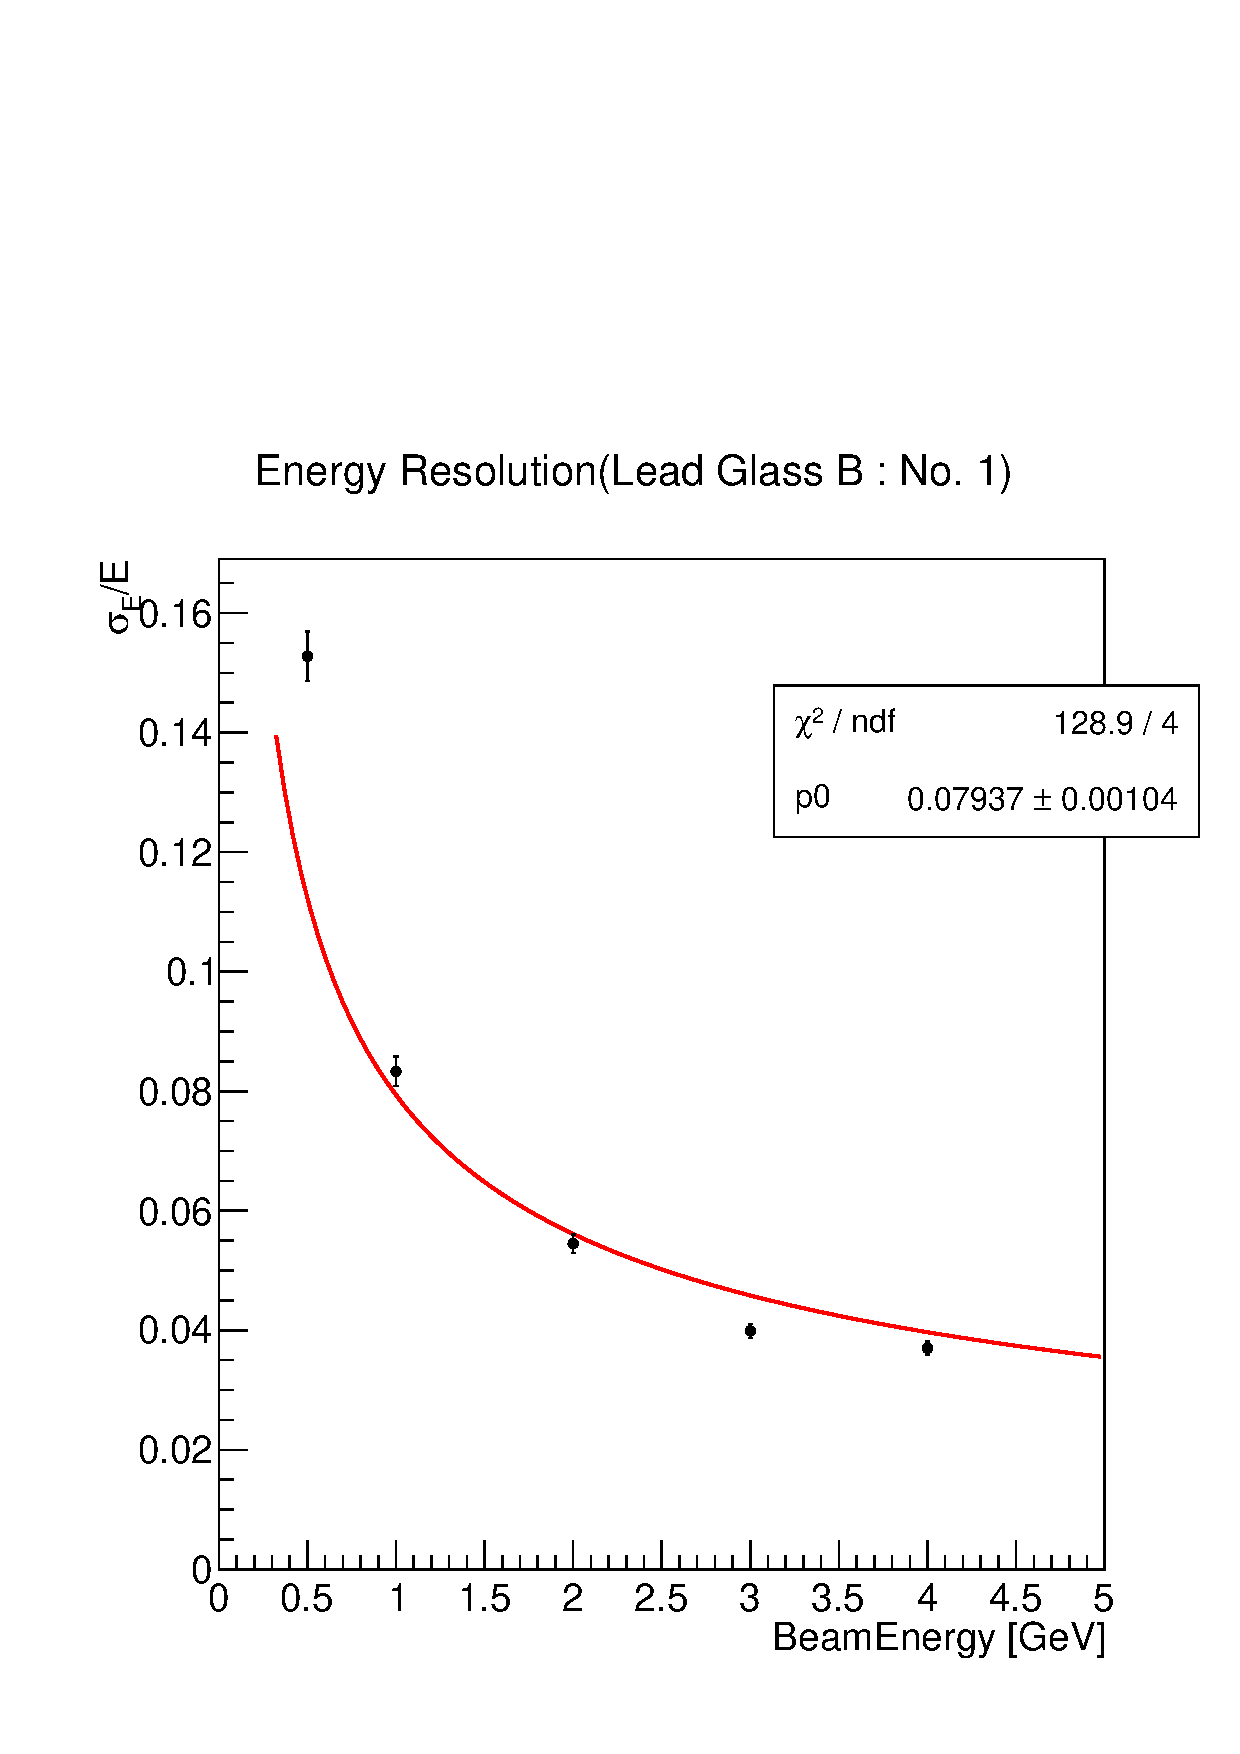
\includegraphics[width=200pt]{./Figure/EBESAnalysis/res_onepara.pdf}%.5\linewidth]{./Figure/DLAnalysis/Input2.png}
			\caption{$p_0$のみによるフィッティング}
			\label{fig:sfig2}
		\end{center}
	\end{subfigure}
	\caption[フィッティングパラメーターの数を変えた比較]{フィッティングパラメーターの数を変えた比較。}
	\label{res_twopara}
\end{figure}

フィッティングパラメータは正の値として得られたが、フィッティングの$\chi^2$値が悪化しており、目視で確認してもデータを適切にフィッティングできていないことがわかる。
次に、低エネルギー$\SI{0.5}{GeV}$のデータを外した上で2パラメータおよび3パラメータでフィッティングを行った。結果を\ref{fitting_wo_low}に示す。

\begin{figure}[H]
	\begin{subfigure}{.5\textwidth}
		\begin{center}
 		 	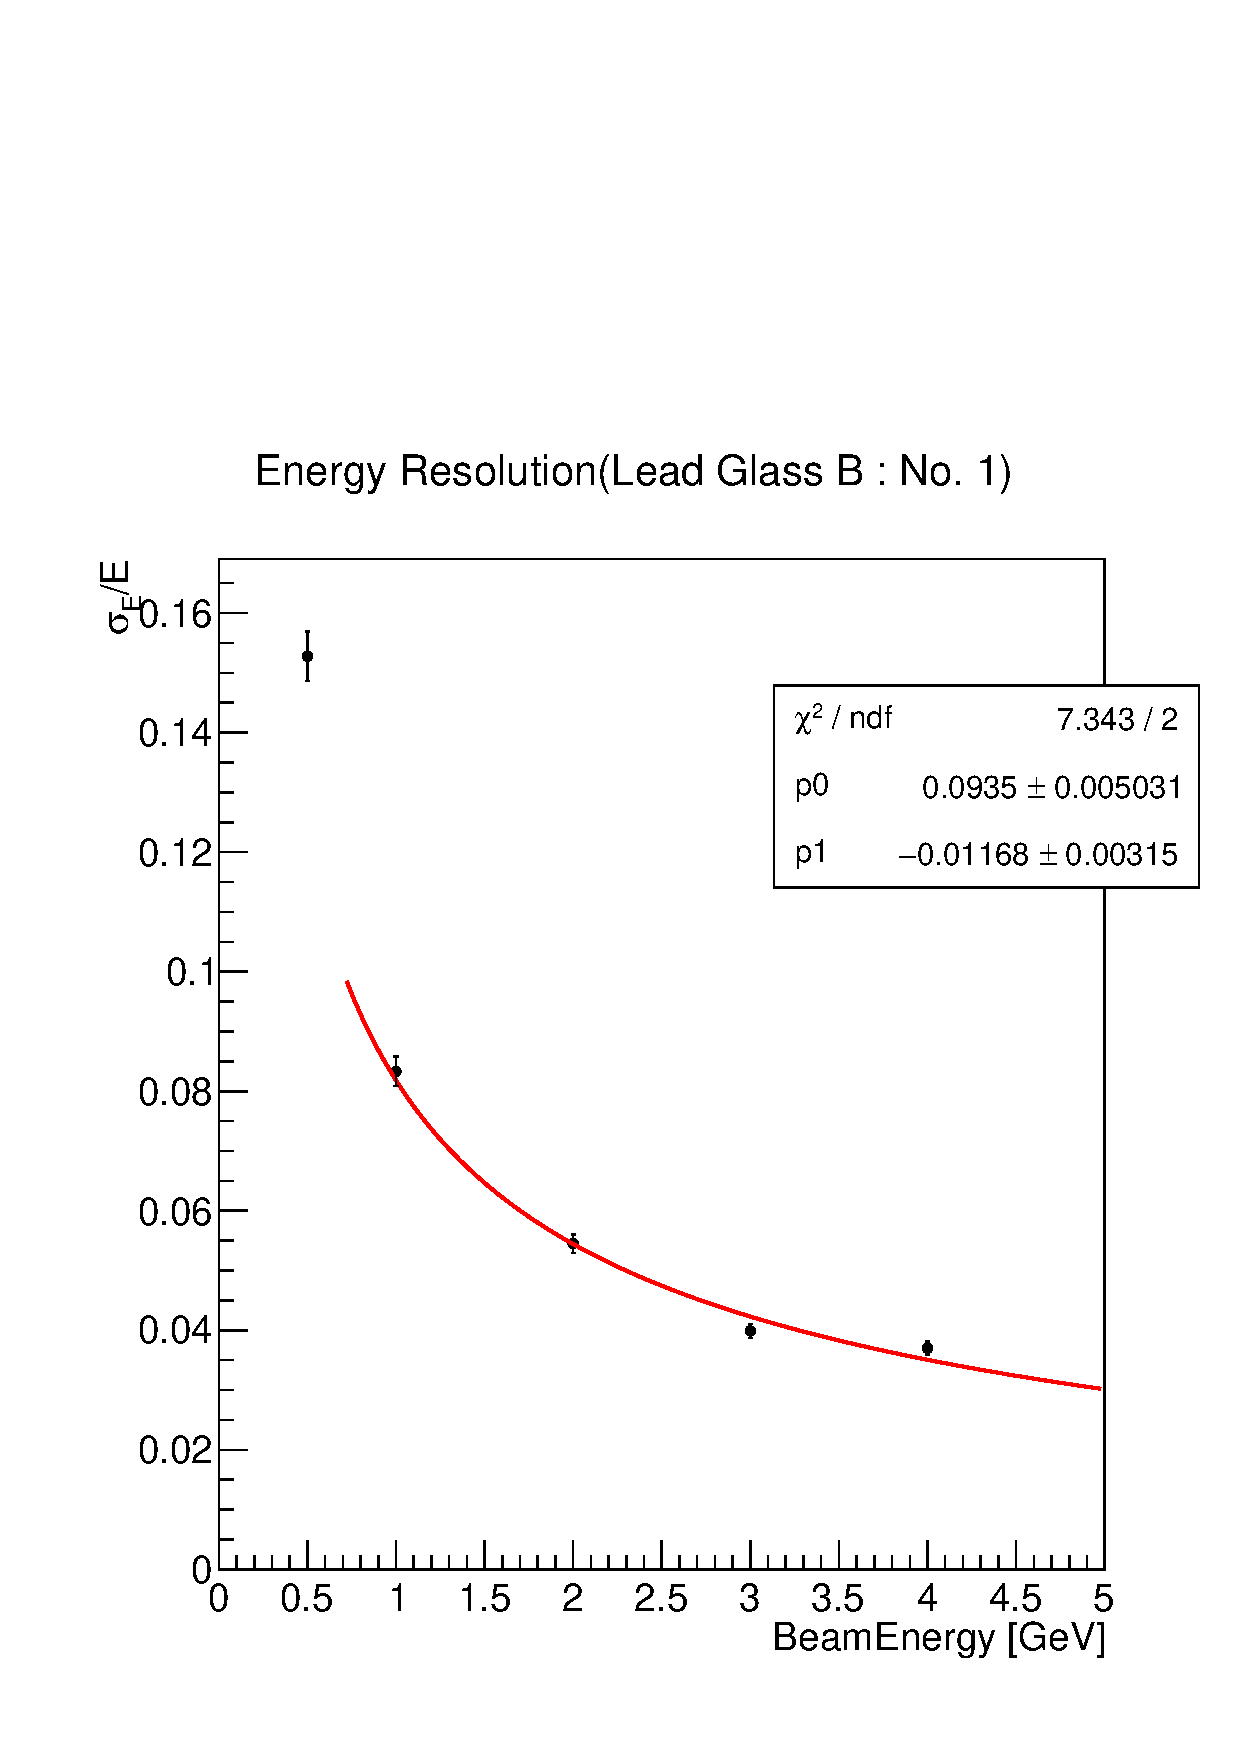
\includegraphics[width=200pt]{./Figure/EBESAnalysis/res_twopara_wo_low.pdf} 
			  \caption{$\SI{0.5}{GeV}$を外した場合の$p_0$および$p_1$によるフィッティング。}
  			\label{fig:sfig1}
 		\end{center}
	\end{subfigure}
	\begin{subfigure}{.5\textwidth}
		\begin{center}
			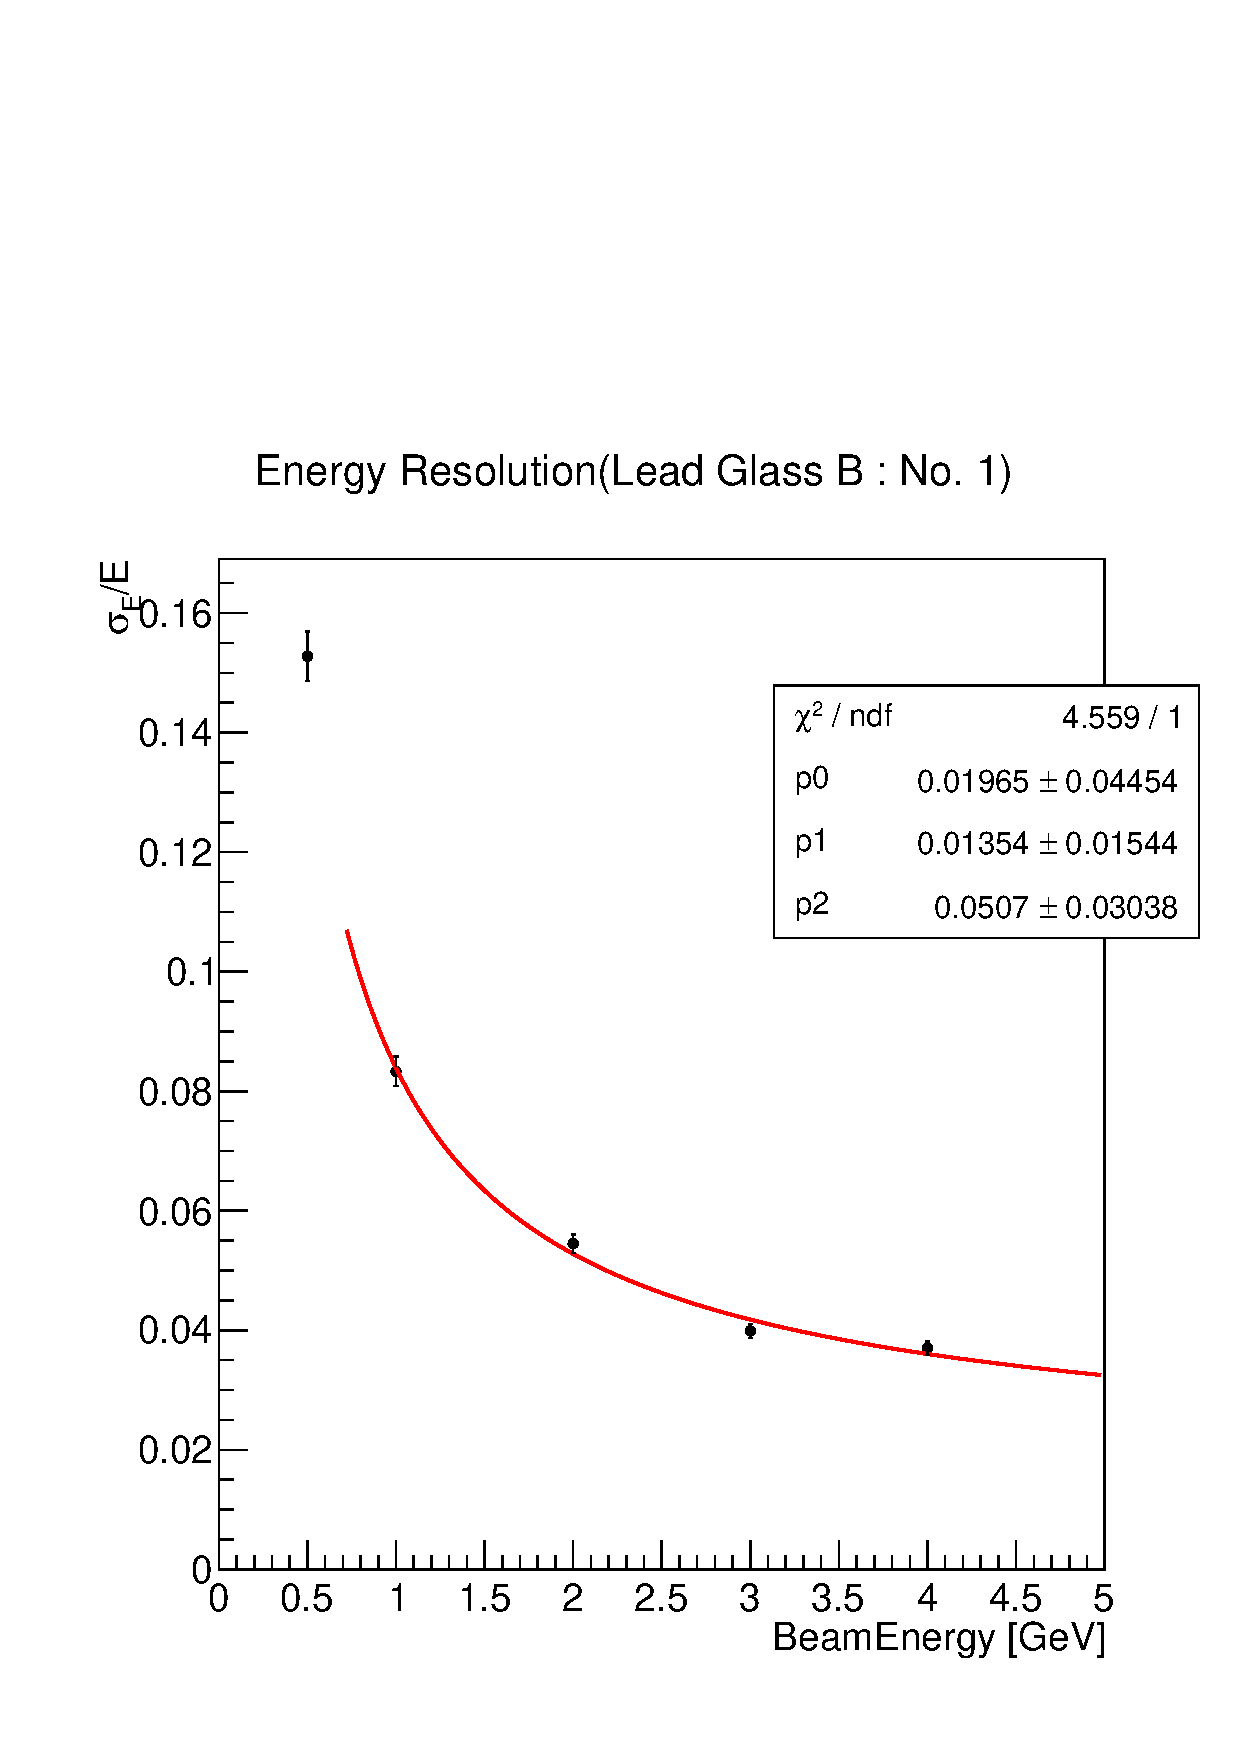
\includegraphics[width=200pt]{./Figure/EBESAnalysis/res_threepara_wo_low.pdf}%.5\linewidth]{./Figure/DLAnalysis/Input2.png}
			\caption{$\SI{0.5}{GeV}$を外した場合の$p_0$、$p_1$、$p_2$によるフィッティング}
			\label{fig:sfig2}
		\end{center}
	\end{subfigure}
	\caption[$\SI{0.5}{GeV}$を外した場合の比較]{$\SI{0.5}{GeV}$を外した場合の比較。}
	\label{fitting_wo_low}
\end{figure}


こちらはさらにフィッティングの$\chi^2$値が改善し、フィッティングパラメータも正の値として得られている。
さらに各項の2乗和の平方根をとった関数
\end{comment}
%%%%%%%%%%%%%%%%%%%%%%%%%%%%%%%%%%%%%%%%%%%%%%%%%%%%%%%%%%%%%%%%%%%%%%%%%%%%%%%%%%%
\begin{equation}
\frac{\sigma}{E} = \sqrt{\left(\frac{p_0}{\sqrt{E}}\right)^2+(p_1)^2 +\left(\frac{p_2}{E}\right)^2}
\end{equation}
と表される。ここで、$p_0$、$p_1$、$p_2$は定数である。それぞれの項は統計項、定数項、ノイズ項と呼ばれる。のちの解析のためにそれぞれの項について詳しく見る。

統計項はビームのエネルギーの平方根に依存して統計的に測定値が揺らぐ統計誤差を表している。鉛ガラス検出器中で発生する光子数は信号電圧に比例し、信号電圧はビームのエネルギーに比例している。一方、統計誤差は光子数の平方根で減少する。したがって、ビームエネルギーが大きくなればその平方根の逆数だけこの項の寄与は減少する。

定数項はビームエネルギーに依存しない系統誤差を表している。例として、検出器の個体差やHVによるものがある。

ノイズ項はビームエネルギーに依存しないノイズを示している。例えば、ペデスタルの影響が挙げられる。ペデスタルは測定されるADCのベースラインとして生じるため、ビームエネルギーが大きくなると共に信号が増大すると、電圧信号(ADC)に対するノイズの割合(S/N比)は改善する。ビームエネルギーはADCと比例関係のため、ビームエネルギーとペデスタルの影響は反比例の関係にある。ノイズ項として現れるのはペデスタルの幅である。図\ref{Pedestal}および図\ref{CorrectBeam}からわかるように、この幅はビームデータの幅よりも小さくなっていることがわかる。

この関数でフィッティングを行った。
結果を図\ref{res_re}に示す。なお、本論文中では検出器1に対して行った解析のみ示している。

\begin{figure}[h]
	\begin{center}
		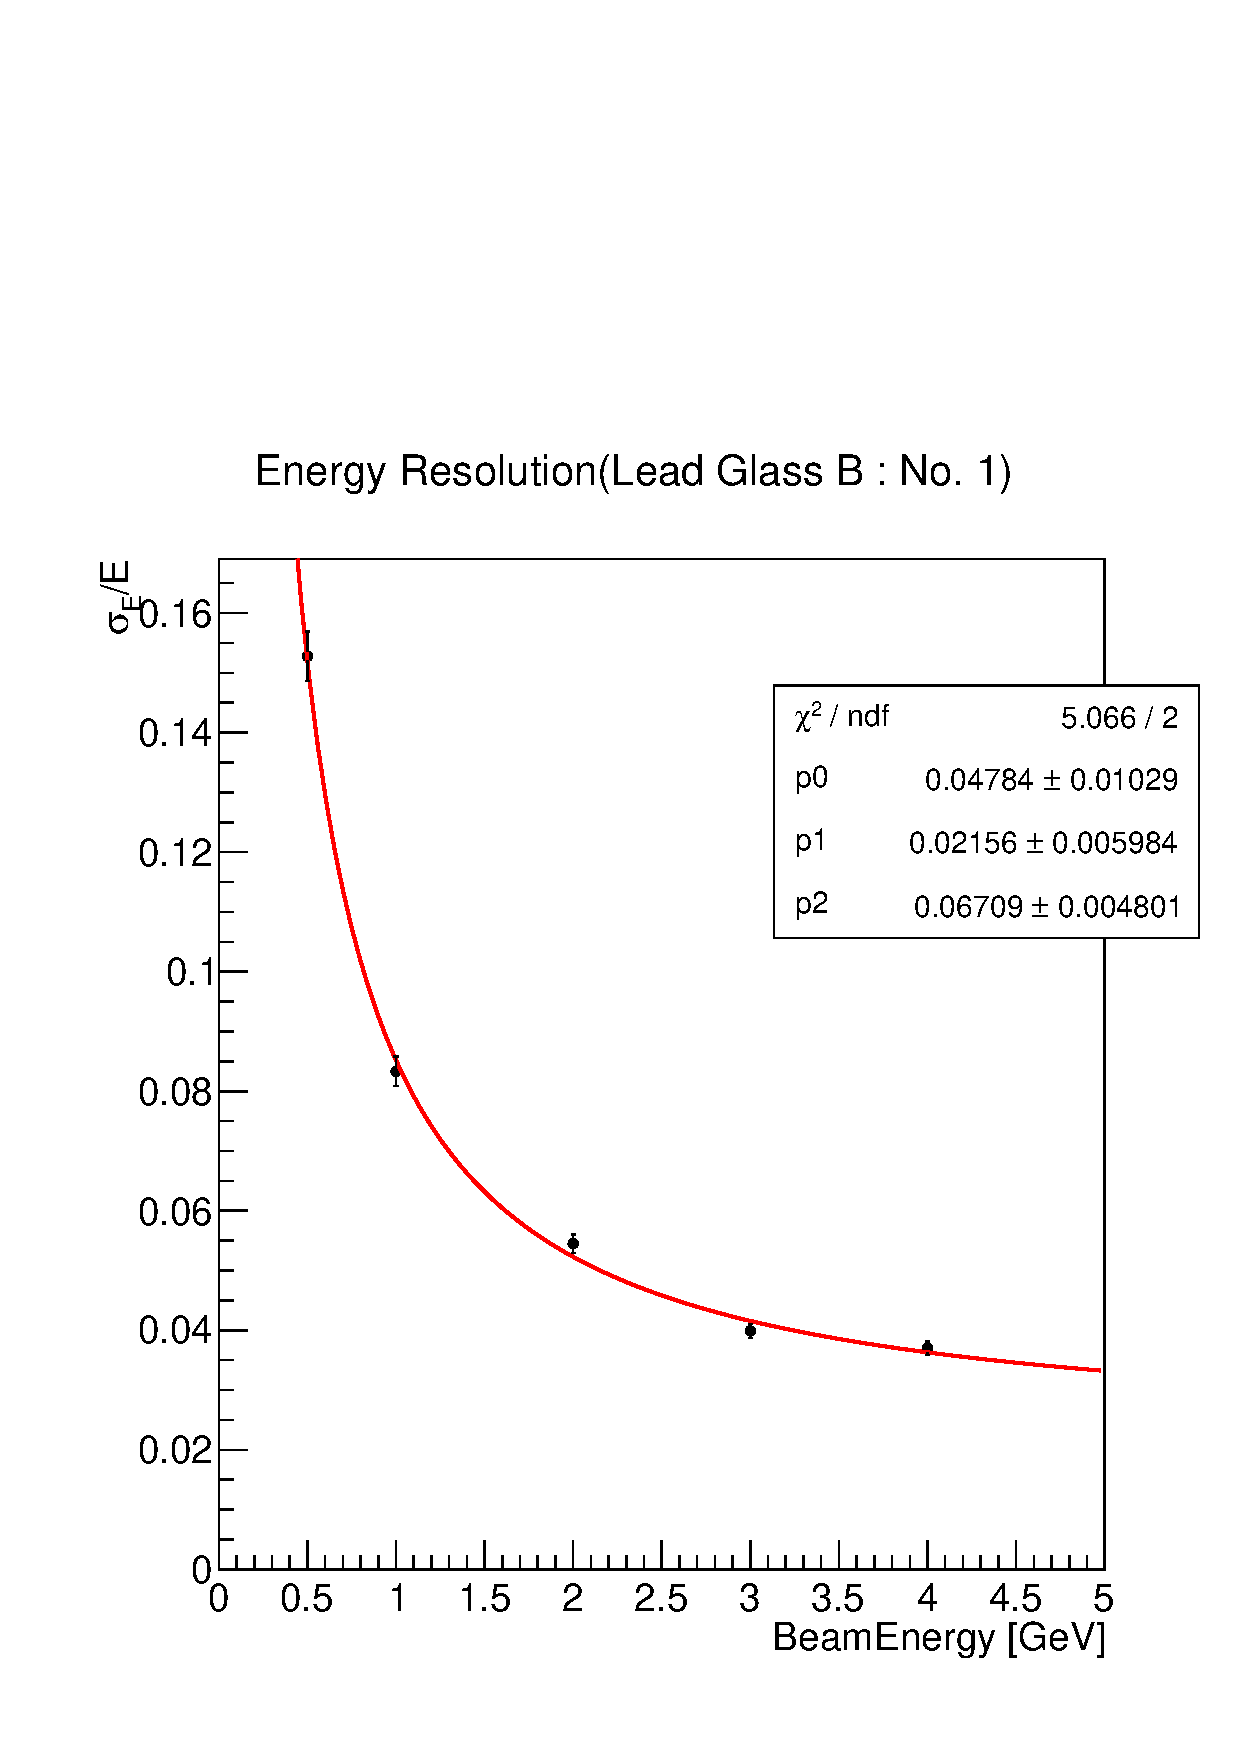
\includegraphics[width=200pt]{./Figure/EBESAnalysis/res_re.pdf}
		\caption[ビームエネルギー分解能のフィッティング]{ビームエネルギー分解能のフィッティング。}
		\label{res_re}
	\end{center}
\end{figure}

フィッティングはデータに対してよく近似できており、$\chi^2$値は後に示すものよりも小さい値となっている一方で、統計項$p_0$がノイズ項$p_2$よりも小さくなっている。しかし一般に、カロリメータの性能として、統計項が通常支配的になる。その上、ペデスタルの幅が十分小さいことと反し、3つのパラメータによるフィットを採用すると実際以上にカロリメータの性能が良いことになってしまう。そのため、フィッティングの条件を変えて最も妥当なプロットを求めた。

まず、フィッティングパラメータの数を変えた場合、およびフィッティング誤差の大きい$\SI{0.5}{GeV}$のデータをフィッティングから除外したものと比較した。
それぞれ、図\ref{res_re_twopara}および\ref{res_re_without_low}に示す。

\begin{figure}[H]
	\begin{subfigure}{.5\textwidth}
		\begin{center}
 		 	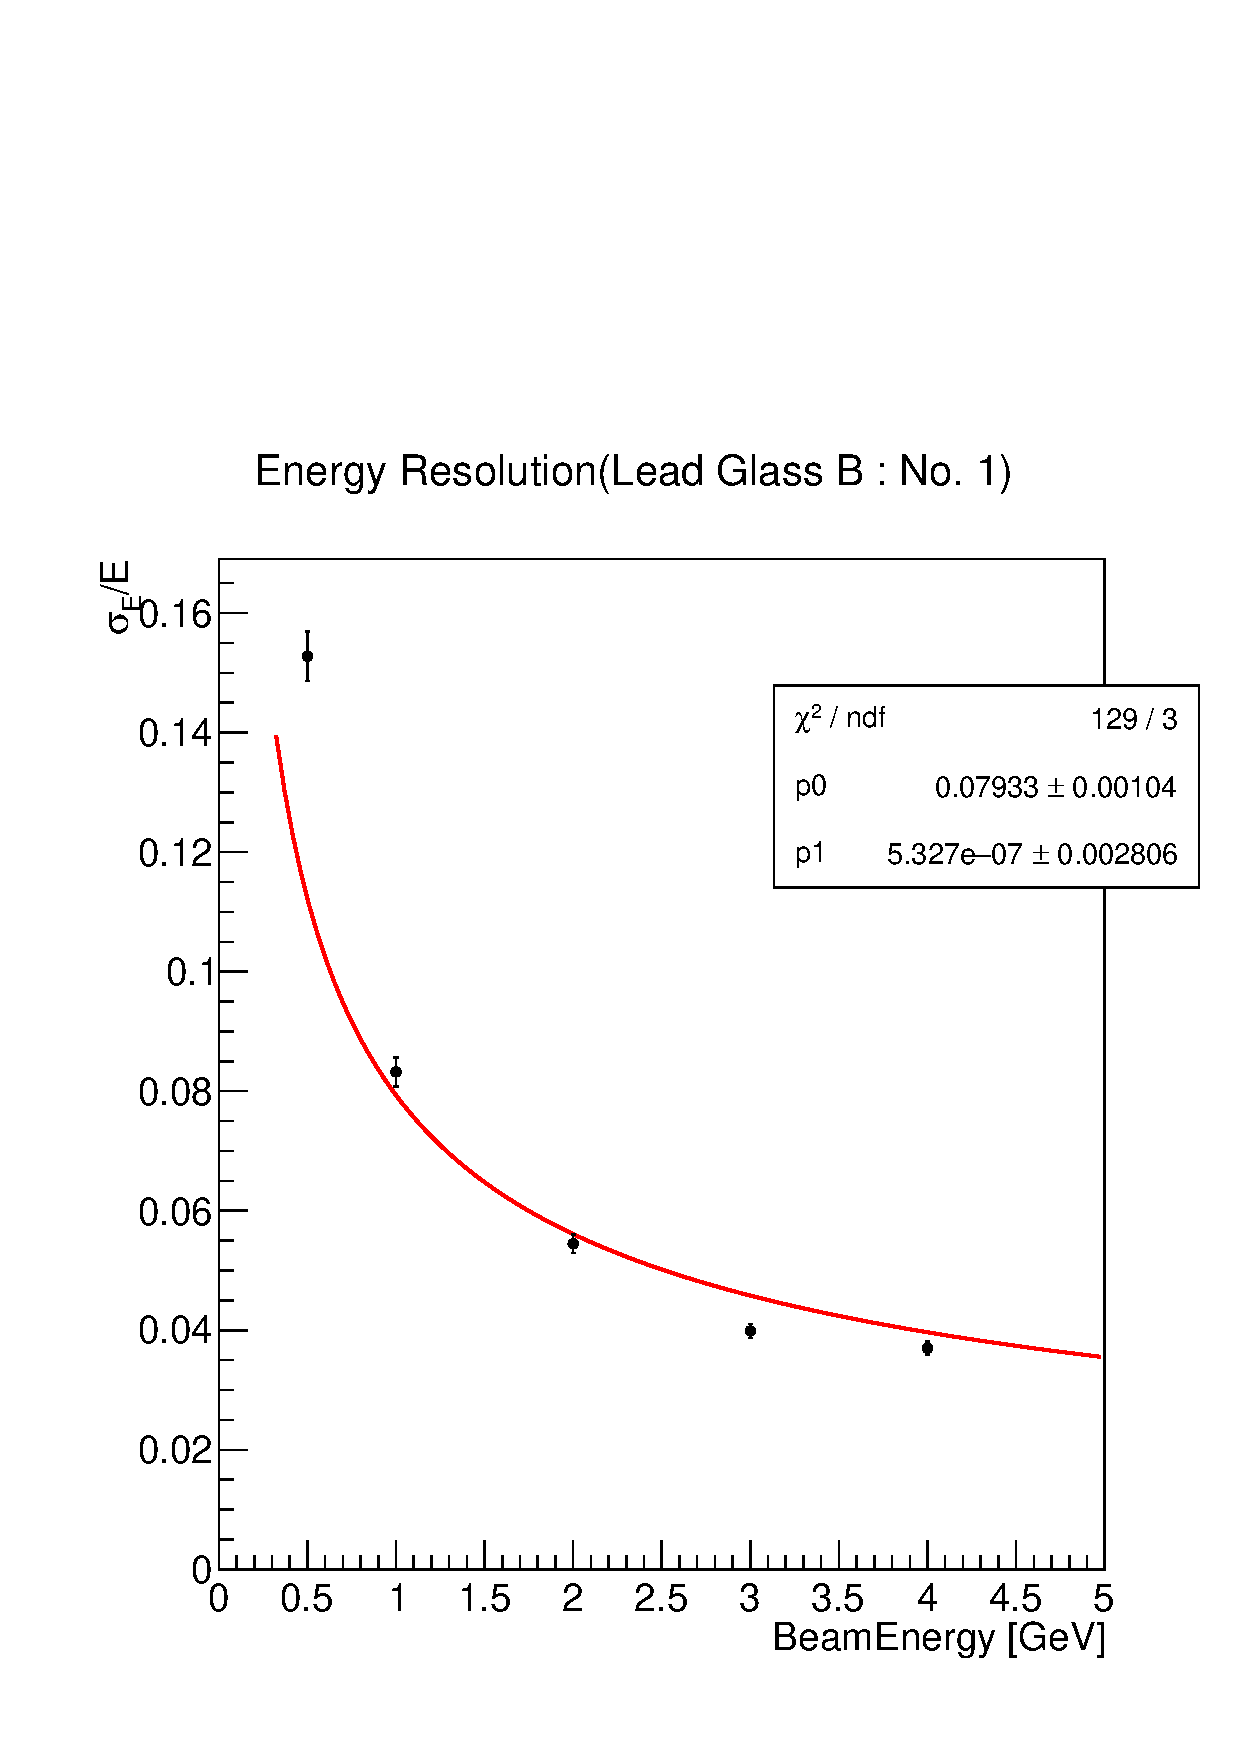
\includegraphics[width=200pt]{./Figure/EBESAnalysis/res_re_twopara.pdf} 
			  \caption{$p_0$および$p_1$によるフィッティング。}
  			\label{fig:sfig1}
 		\end{center}
	\end{subfigure}
	\begin{subfigure}{.5\textwidth}
		\begin{center}
			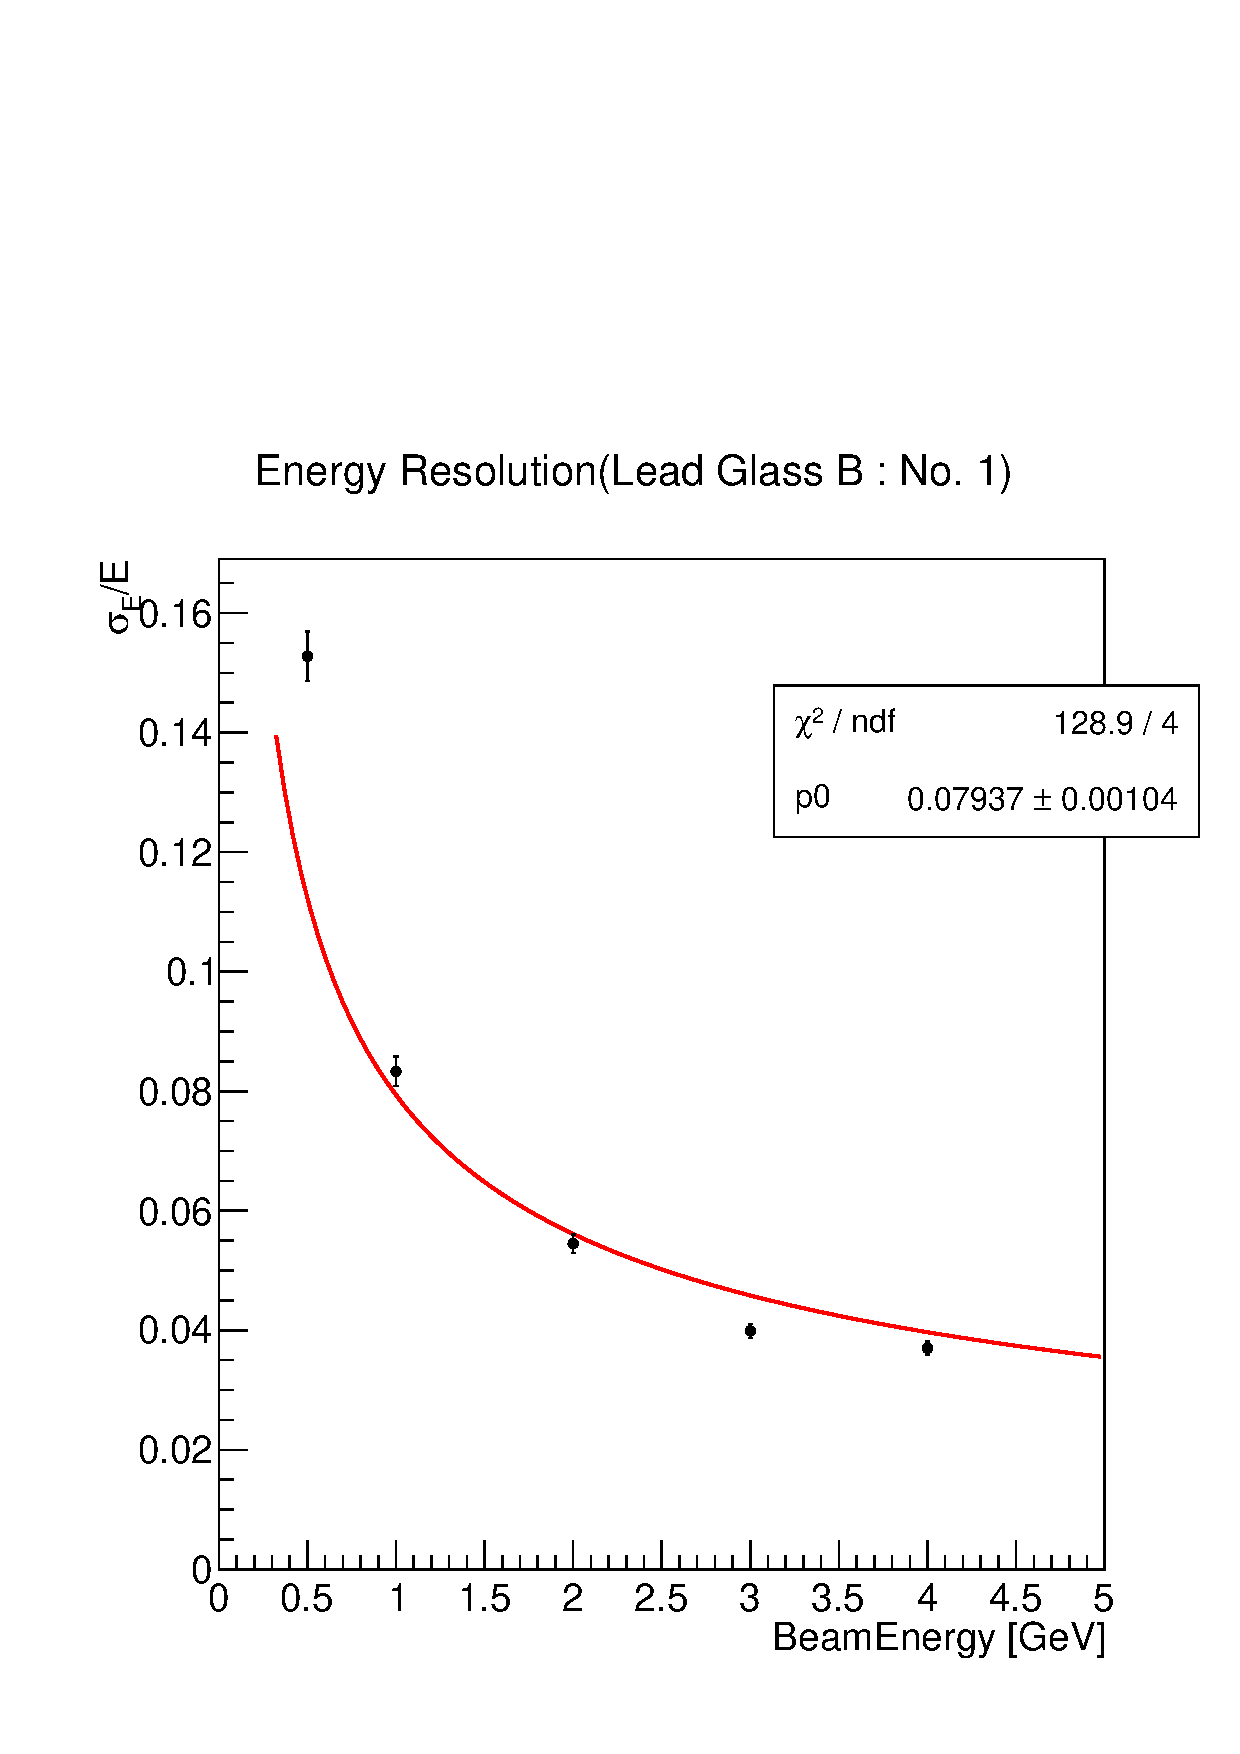
\includegraphics[width=200pt]{./Figure/EBESAnalysis/res_onepara.pdf}%.5\linewidth]{./Figure/DLAnalysis/Input2.png}
			\caption{$p_0$によるフィッティング。$p_1$および$p_2$は0に固定した。}
			\label{fig:sfig2}
		\end{center}
	\end{subfigure}
	\caption[フィッティングパラメータの数を変えた場合の比較]{フィッティングパラメータの数を変えた場合の比較。}
	\label{res_re_twopara}
\end{figure}

\begin{figure}[H]
	\begin{subfigure}{.5\textwidth}
		\begin{center}
 		 	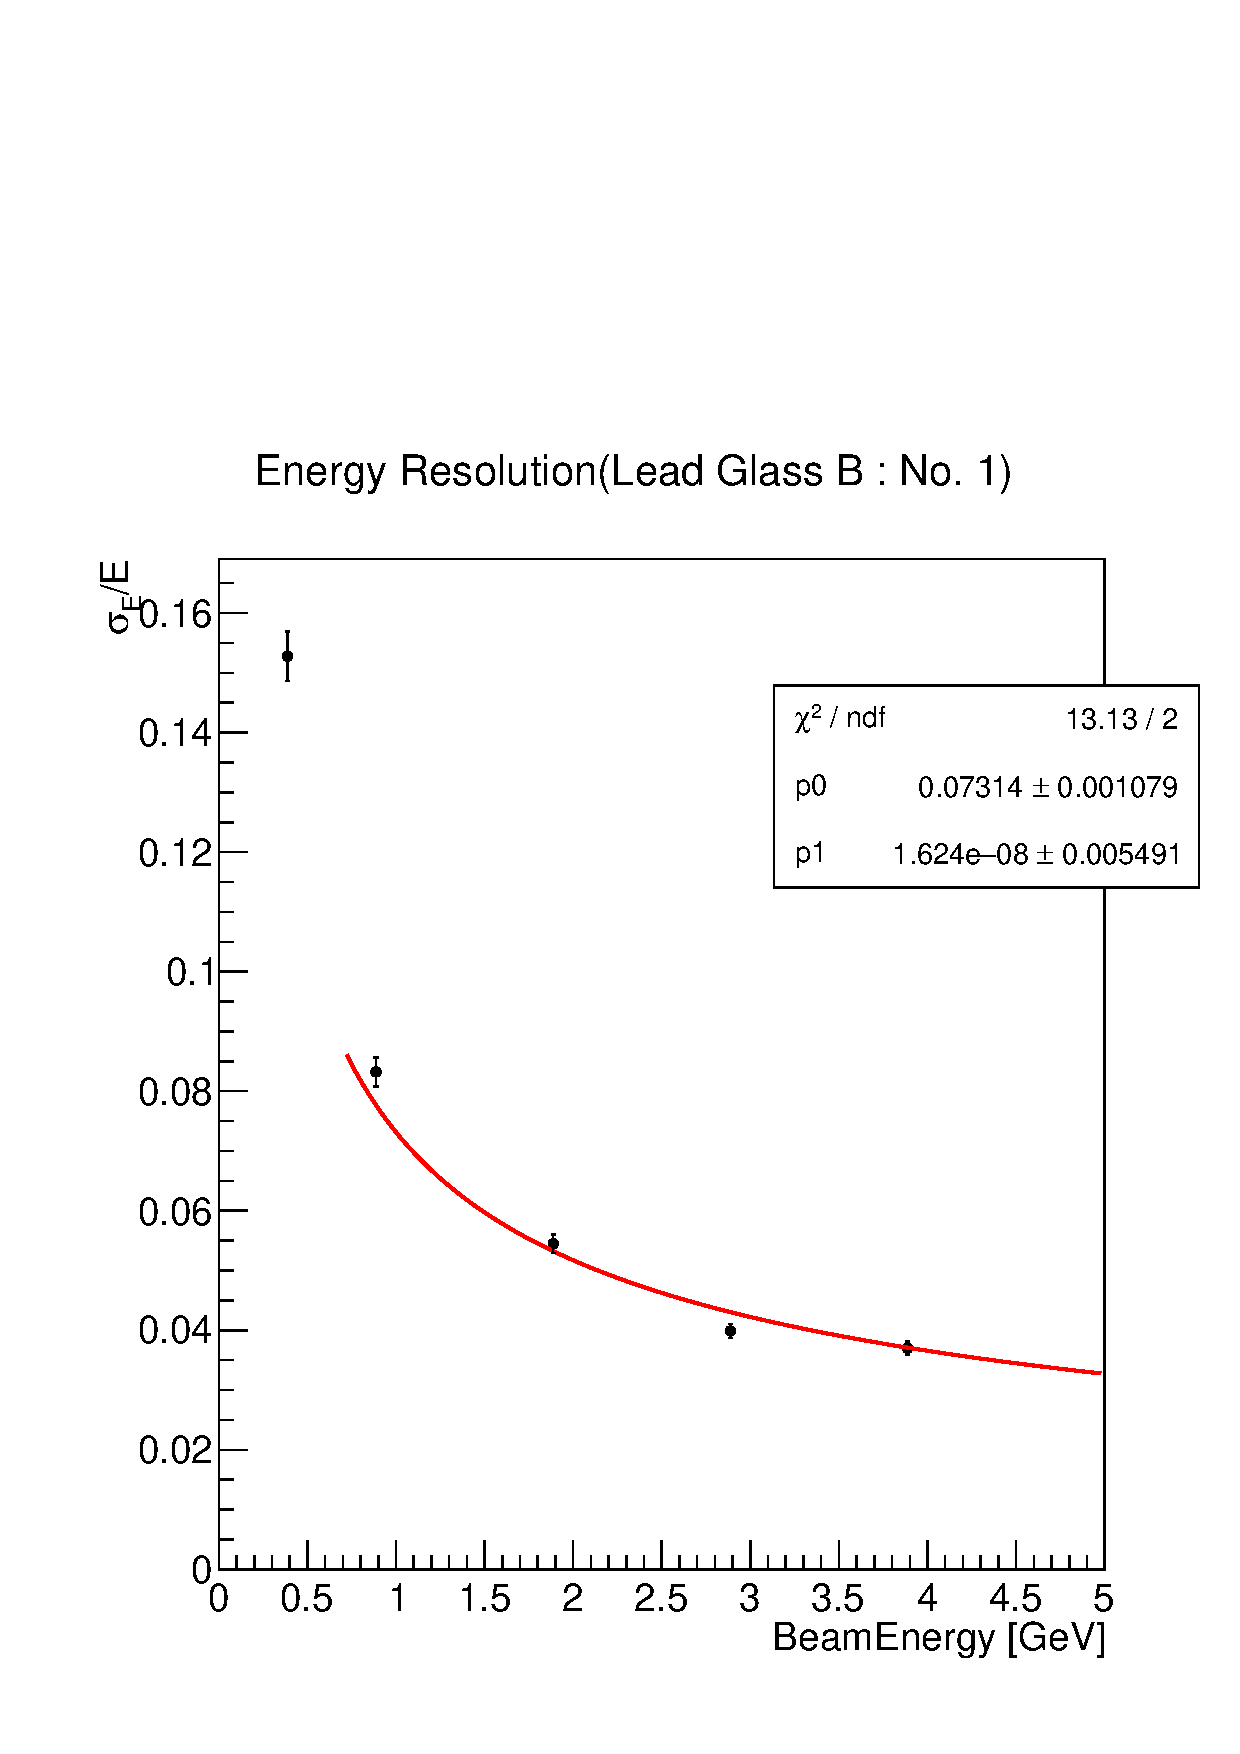
\includegraphics[width=200pt]{./Figure/EBESAnalysis/res_re_twopara_without_low.pdf} 
			  \caption{$p_0$および$p_1$によるフィッティング。}
  			\label{fig:sfig1}
 		\end{center}
	\end{subfigure}
	\begin{subfigure}{.5\textwidth}
		\begin{center}
			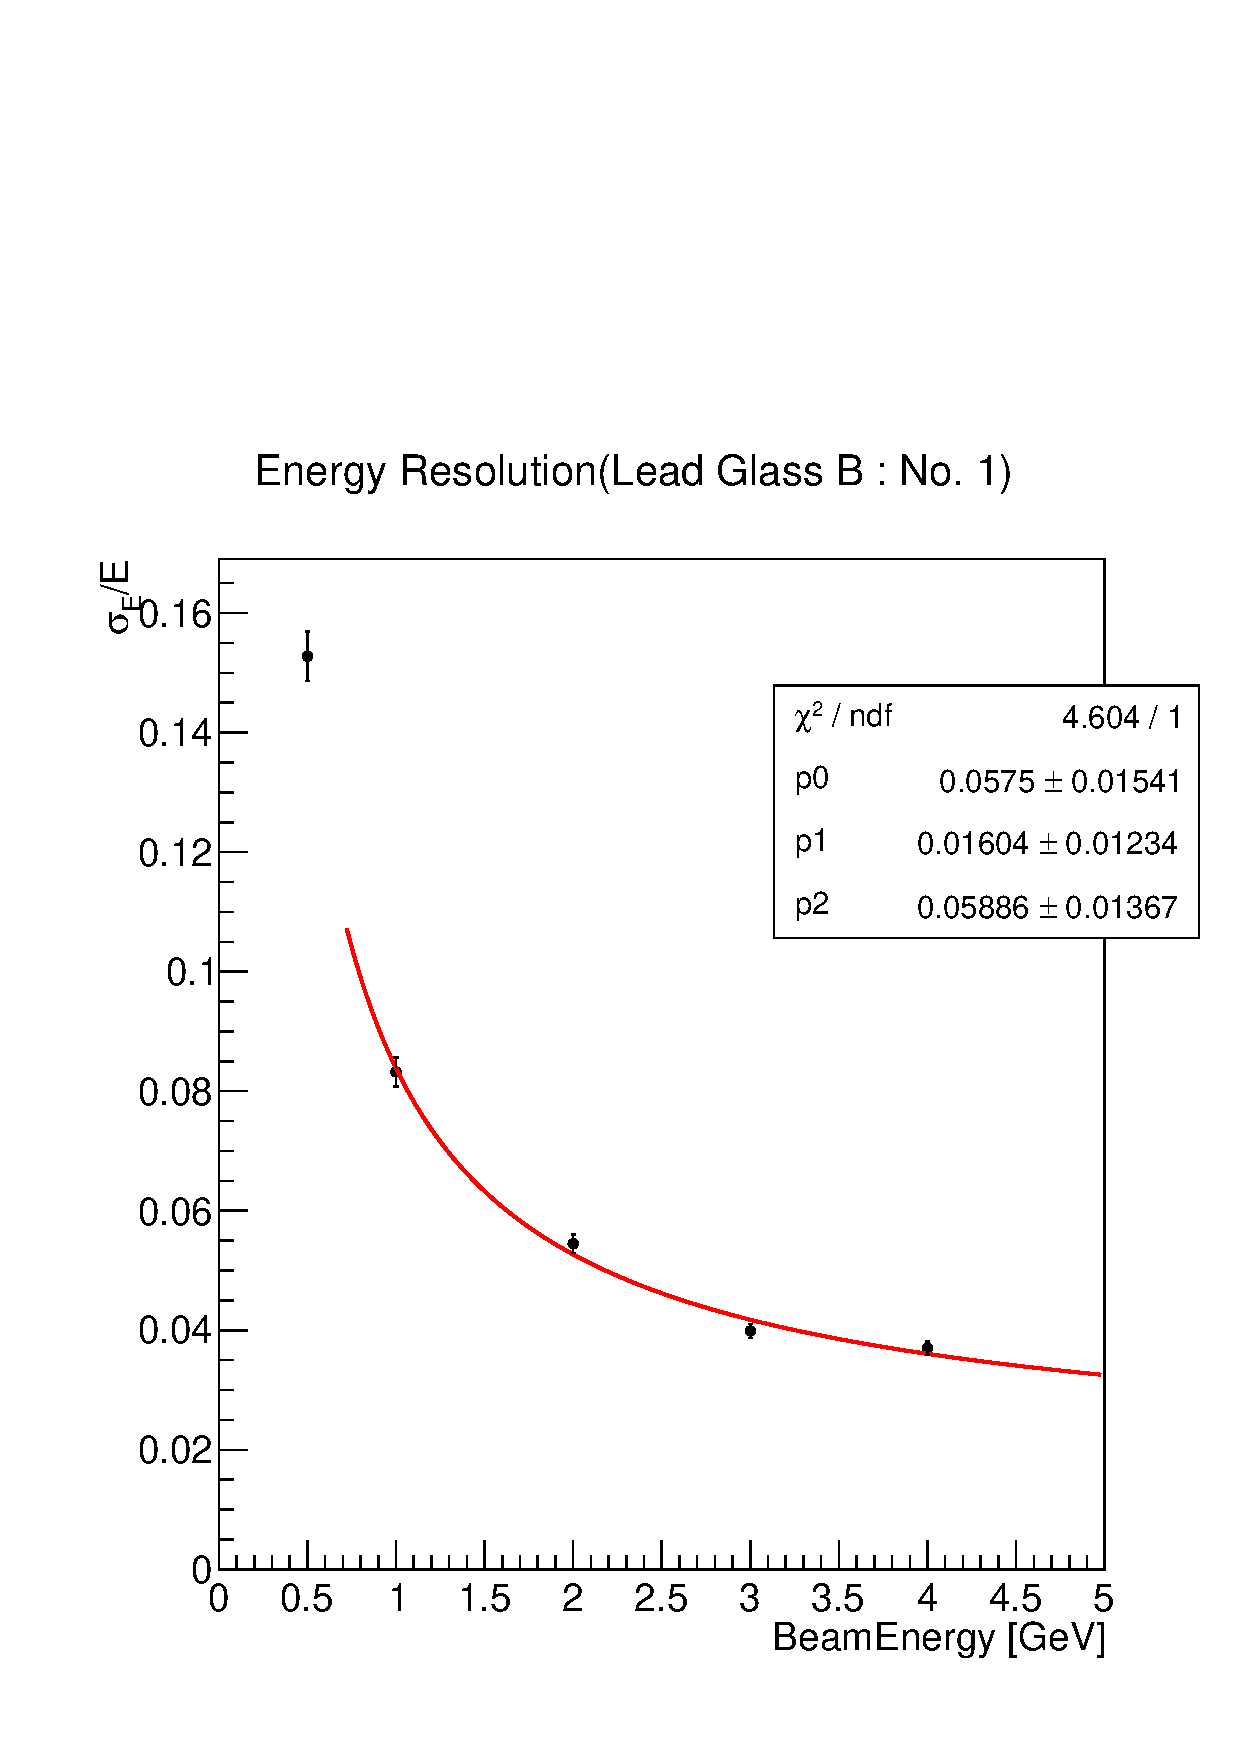
\includegraphics[width=200pt]{./Figure/EBESAnalysis/res_re_threepara_without_low.pdf}%.5\linewidth]{./Figure/DLAnalysis/Input2.png}
			\caption{$p_0$、$p_1$、$p_2$によるフィッティング。}
			\label{fig:sfig2}
		\end{center}
	\end{subfigure}
	\caption[$\SI{0.5}{GeV}$を外した場合の比較。]{$\SI{0.5}{GeV}$を外した場合の比較。}
	\label{res_re_without_low}
\end{figure}

フィッティングパラメータを2つに変更すると、$\chi^2$値は悪化したが、$p_0$は増加した。さらに、\SI{0.5}{GeV}の点を外したときのフィッティングを見ると、フィッティングパラメータが2つのプロットは$\chi^2$が大きく改善している一方で3つのものはやはり$\chi^2$値は良いものの、$p_2$が$p_0$を上回っている。

最後に、$x$切片の平均を考慮することで得られたビームエネルギーの補正を加えてフィッティングを行った。
その結果を図\ref{res_re_fixbeam}に示す。
\begin{figure}[H]
	\begin{subfigure}{.5\textwidth}
		\begin{center}
 		 	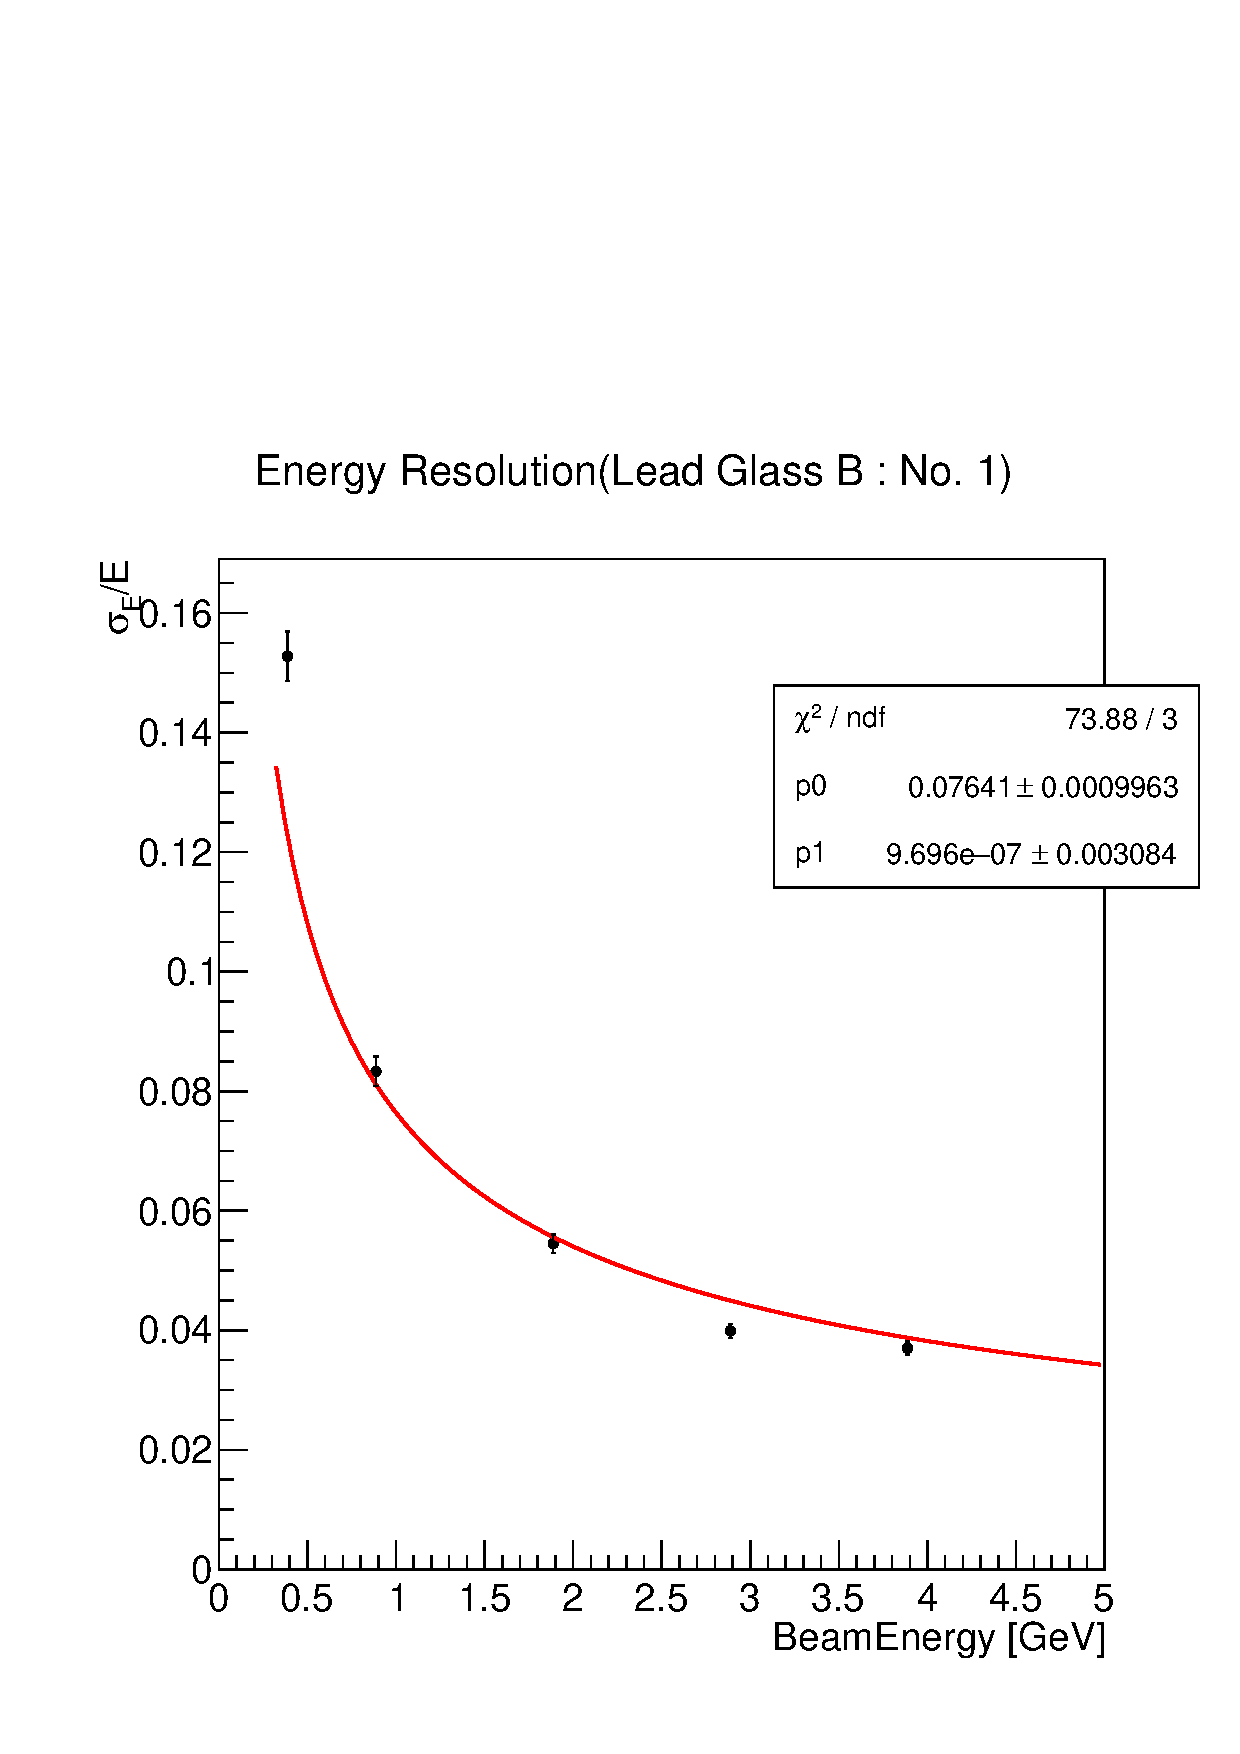
\includegraphics[width=200pt]{./Figure/EBESAnalysis/res_re_twopara_fixbeam.pdf} 
			  \caption{$p_0$および$p_1$によるフィッティング。}
  			\label{fig:sfig1}
 		\end{center}
	\end{subfigure}
	\begin{subfigure}{.5\textwidth}
		\begin{center}
			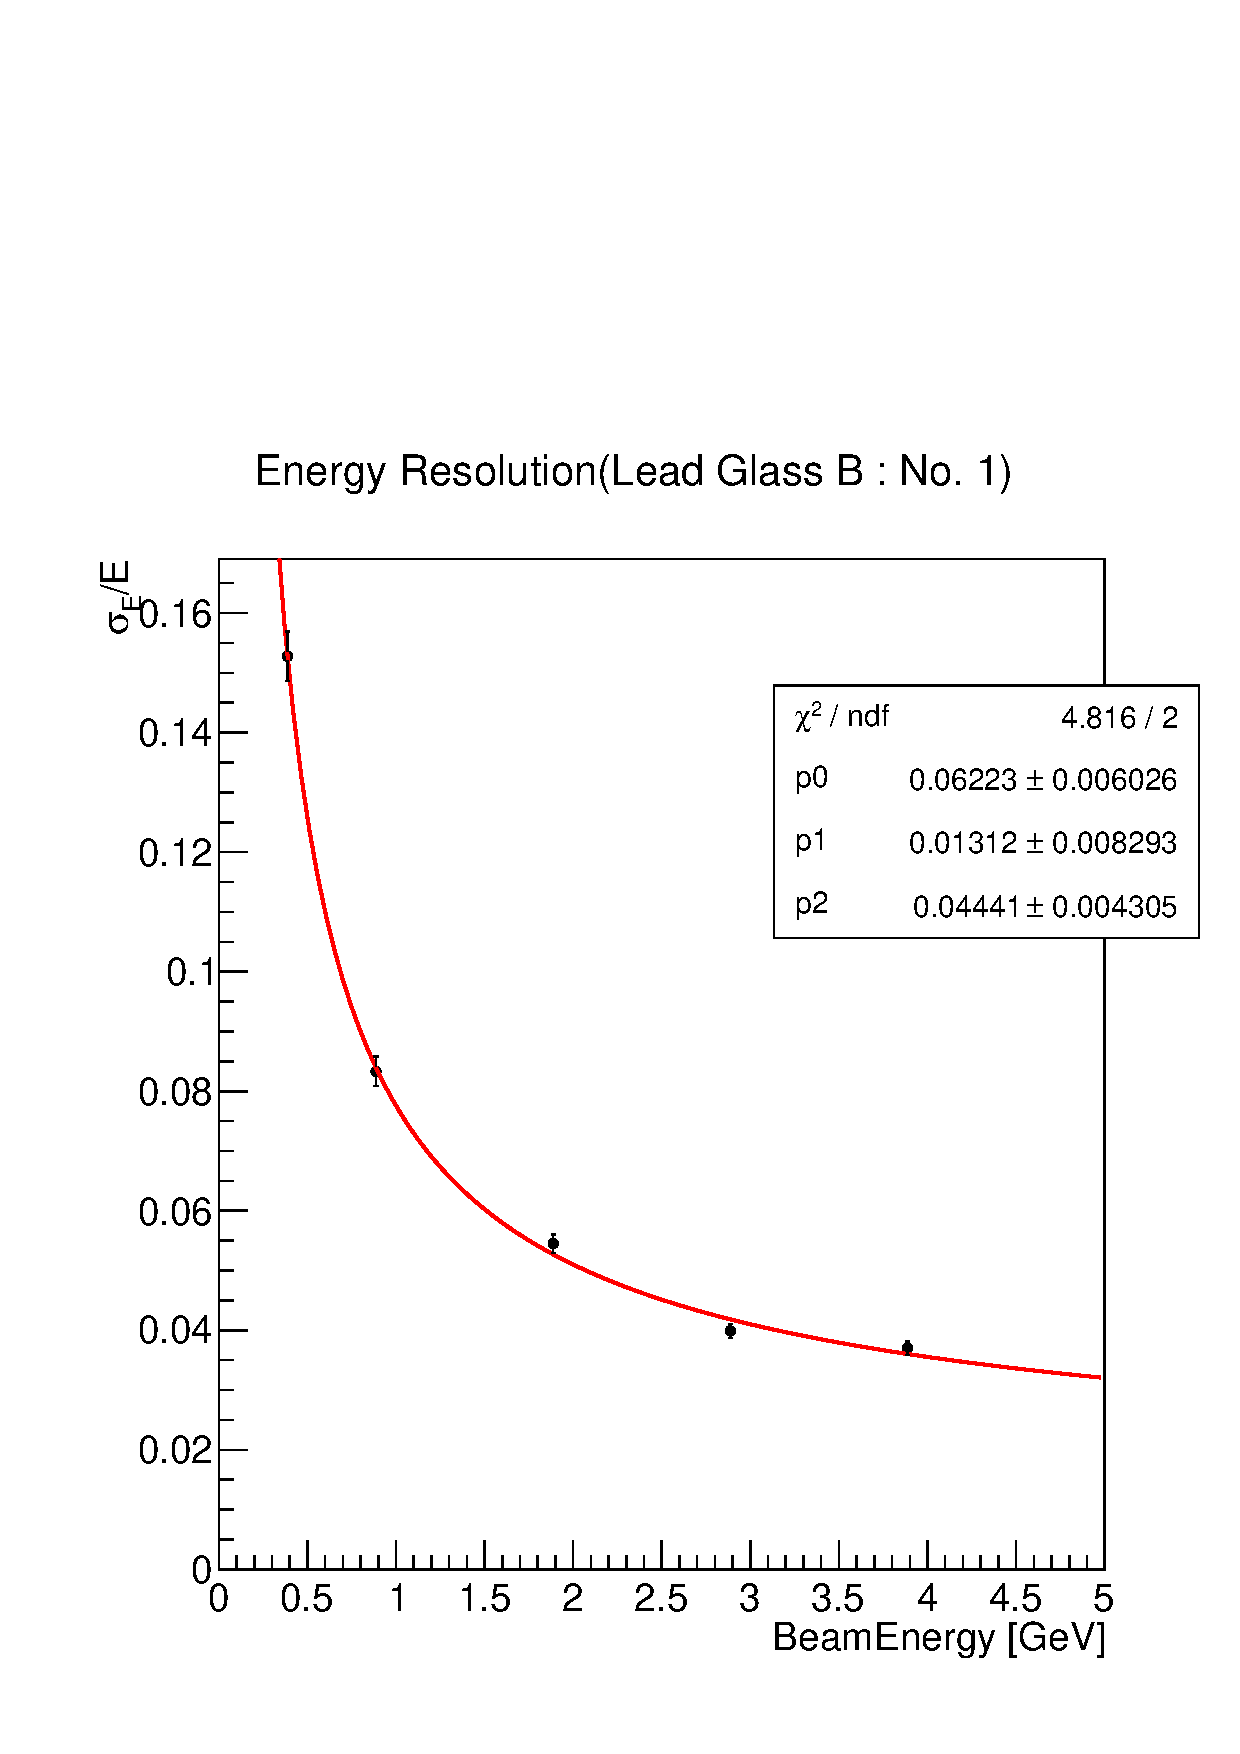
\includegraphics[width=200pt]{./Figure/EBESAnalysis/res_re_threepara_fixbeam.pdf}%.5\linewidth]{./Figure/DLAnalysis/Input2.png}
			\caption{$p_0$、$p_1$、$p_2$によるフィッティング。}
			\label{fig:sfig2}
		\end{center}
	\end{subfigure}
	\caption[ビームエネルギーの補正を行った場合の比較。]{ビームエネルギーの補正を行った場合の比較。}
	\label{res_re_fixbeam}
\end{figure}

\SI{0.5}{GeV}を外した場合と比較すると、$\chi^2$値は悪化している。しかし、図\ref{res_re}および\ref{res_re_twopara}よりは$\chi^2$値は改善している。

以上の結果から、検出器1のエネルギー分解能として、\SI{0.5}{GeV}を外した上でパラメータ2つでフィッティングを行なった場合の値を採用した。この場合、
\begin{equation}
\sigma_E/E\approx 7.3/\sqrt{E}\%
\end{equation}
と推計される。

以前TRISTAN実験において測定された時のプロットを図\ref{TRISTAN}に示す~\cite{LeadGlass}。この際のエネルギー分解能はおよそ3\%/$\sqrt{E}$、5\%/$\sqrt{E}$、5.8\%/$\sqrt{E}$であり、今回の結果はその時点よりも悪化していることを示している。原因としては、PMTの経年劣化や鉛ガラスの濁りなどが挙げられる。一方で、今回の実験で想定されたエネルギー分解能は15\%/$\sqrt{E}$であり、シミュレーションもこの値に基づいて行われている。今回得られた結果はこの値を達成しており、本実験に用いるために十分な性能を持っているといえる。

\begin{figure}[H]
	\begin{center}
		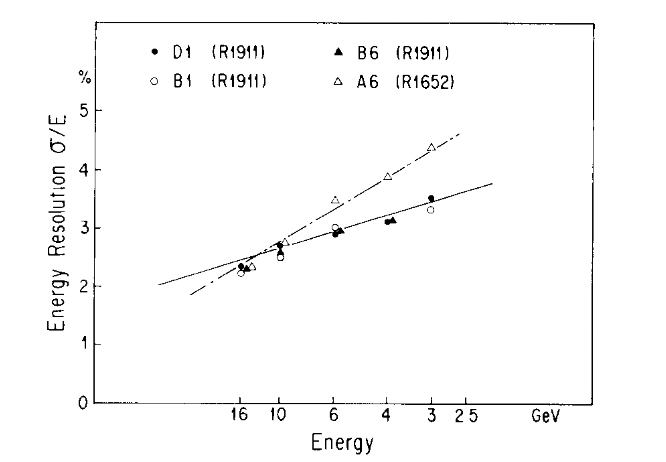
\includegraphics[width=200pt]{./Figure/EBESAnalysis/TRISTAN.png}
		\caption[TRISTAN実験におけるビームエネルギー分解能のフィッティング]{TRISTAN実験におけるビームエネルギー分解能のフィッティング。それぞれの点は検出器につけられたラベルの違いを示している。}
		\label{TRISTAN}
	\end{center}
\end{figure}


また、ビームエネルギーの補正を行なった結果、ADCとビームエネルギーの線形性が回復したことや、エネルギー分解能のフィッティングの$\chi^2$値が改善したことなどから、実際のビームエネルギーにズレが生じている可能性がある。今後更なる実験を行い、この点については検証する必要があると考えられる。

\section{HVを変えた際の検出器応答の変化}

ビームテスト開始時に、ビームエネルギーを$\SI{5.0}{GeV}$に固定した上でPMTに印加するHVを$\SI{-1450}{V}$から$\SI{-1700}{V}$へ変えてADCを測定した。この測定はバックグラウンド測定実験において得られたデータから、検出器内で生じたエネルギーを見積もるために測定を行った。このデータに対して$V$を印加電圧として、
\begin{equation}
f(V) = p_0 V^{p_1}
\end{equation}
によってフィッティングを行った。図\ref{HVscan}にその結果を示す。ただし、電圧値は絶対値で表記している。

\begin{figure}[H]
	\begin{center}
		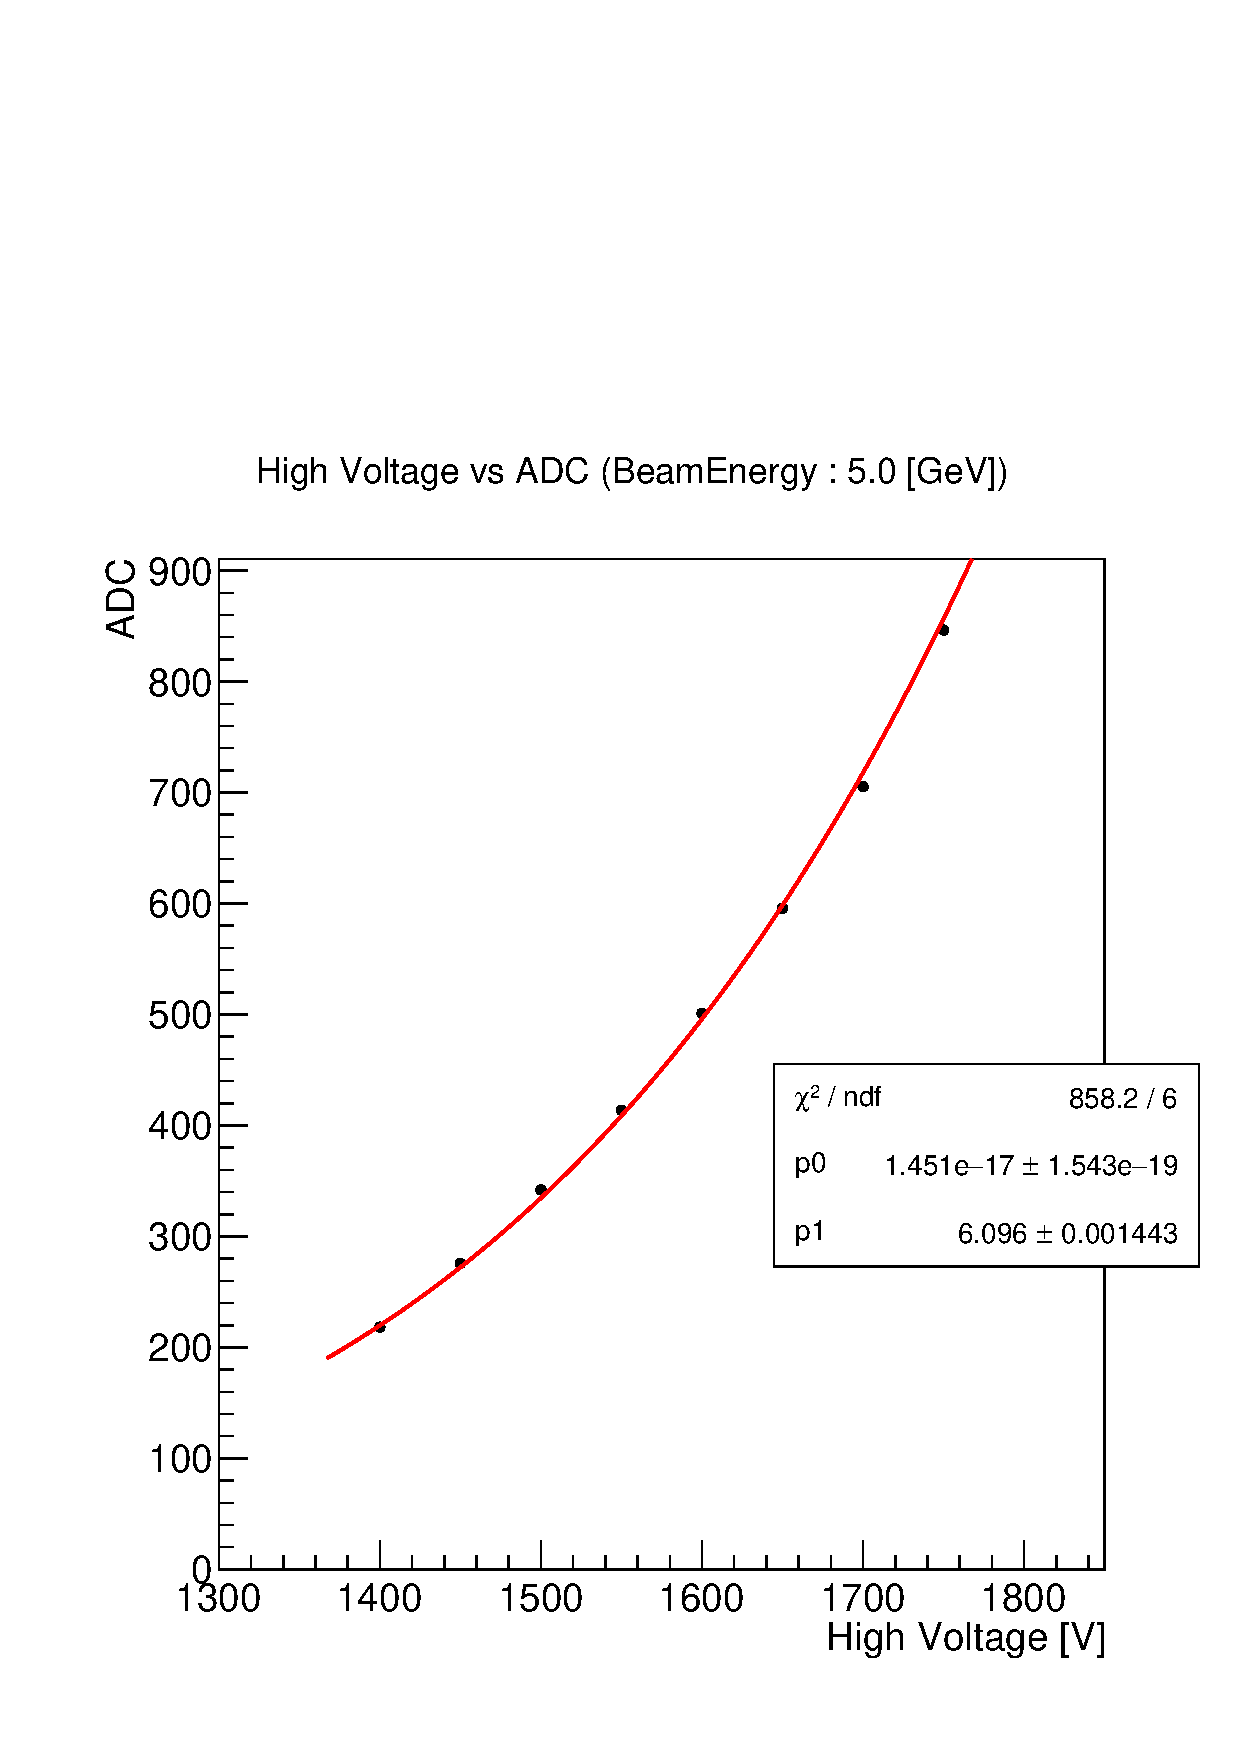
\includegraphics[width=200pt]{./Figure/EBESAnalysis/HVscan.pdf}
		\caption[PMTに印加したHVとADCの関係]{PMTに印加したHVとADCの関係。}
		\label{HVscan}
	\end{center}
\end{figure}

この関数はPMTの印加電圧に対する増幅率(ゲイン)に基づいていると考えられる。PMT内において、光子が1つの電極に衝突した後に放出される光電子のエネルギーは電極間の電圧$V$に比例するため、この増幅率を表す二次電子放出係数$\delta$は比例定数を$K$として、
\begin{equation}
\delta = KV
\end{equation}
と表される。PMT内に$n$個の光電面が存在するとすると、全体のゲイン$G$は
\begin{equation}
G=\delta^n=(KV)^n
\end{equation}
となる。ただし、実際の性能は個体差があるため、フィッティングによる見積もりが必要となる。

フィッティングによって得られた曲線をバックグラウンド測定の際に鉛ガラス検出器に印加した$\SI{850}{V}$におけるADCを得るために原点まで外挿した。外挿曲線を図\ref{extra}に示す。
\begin{figure}[H]
	\begin{center}
		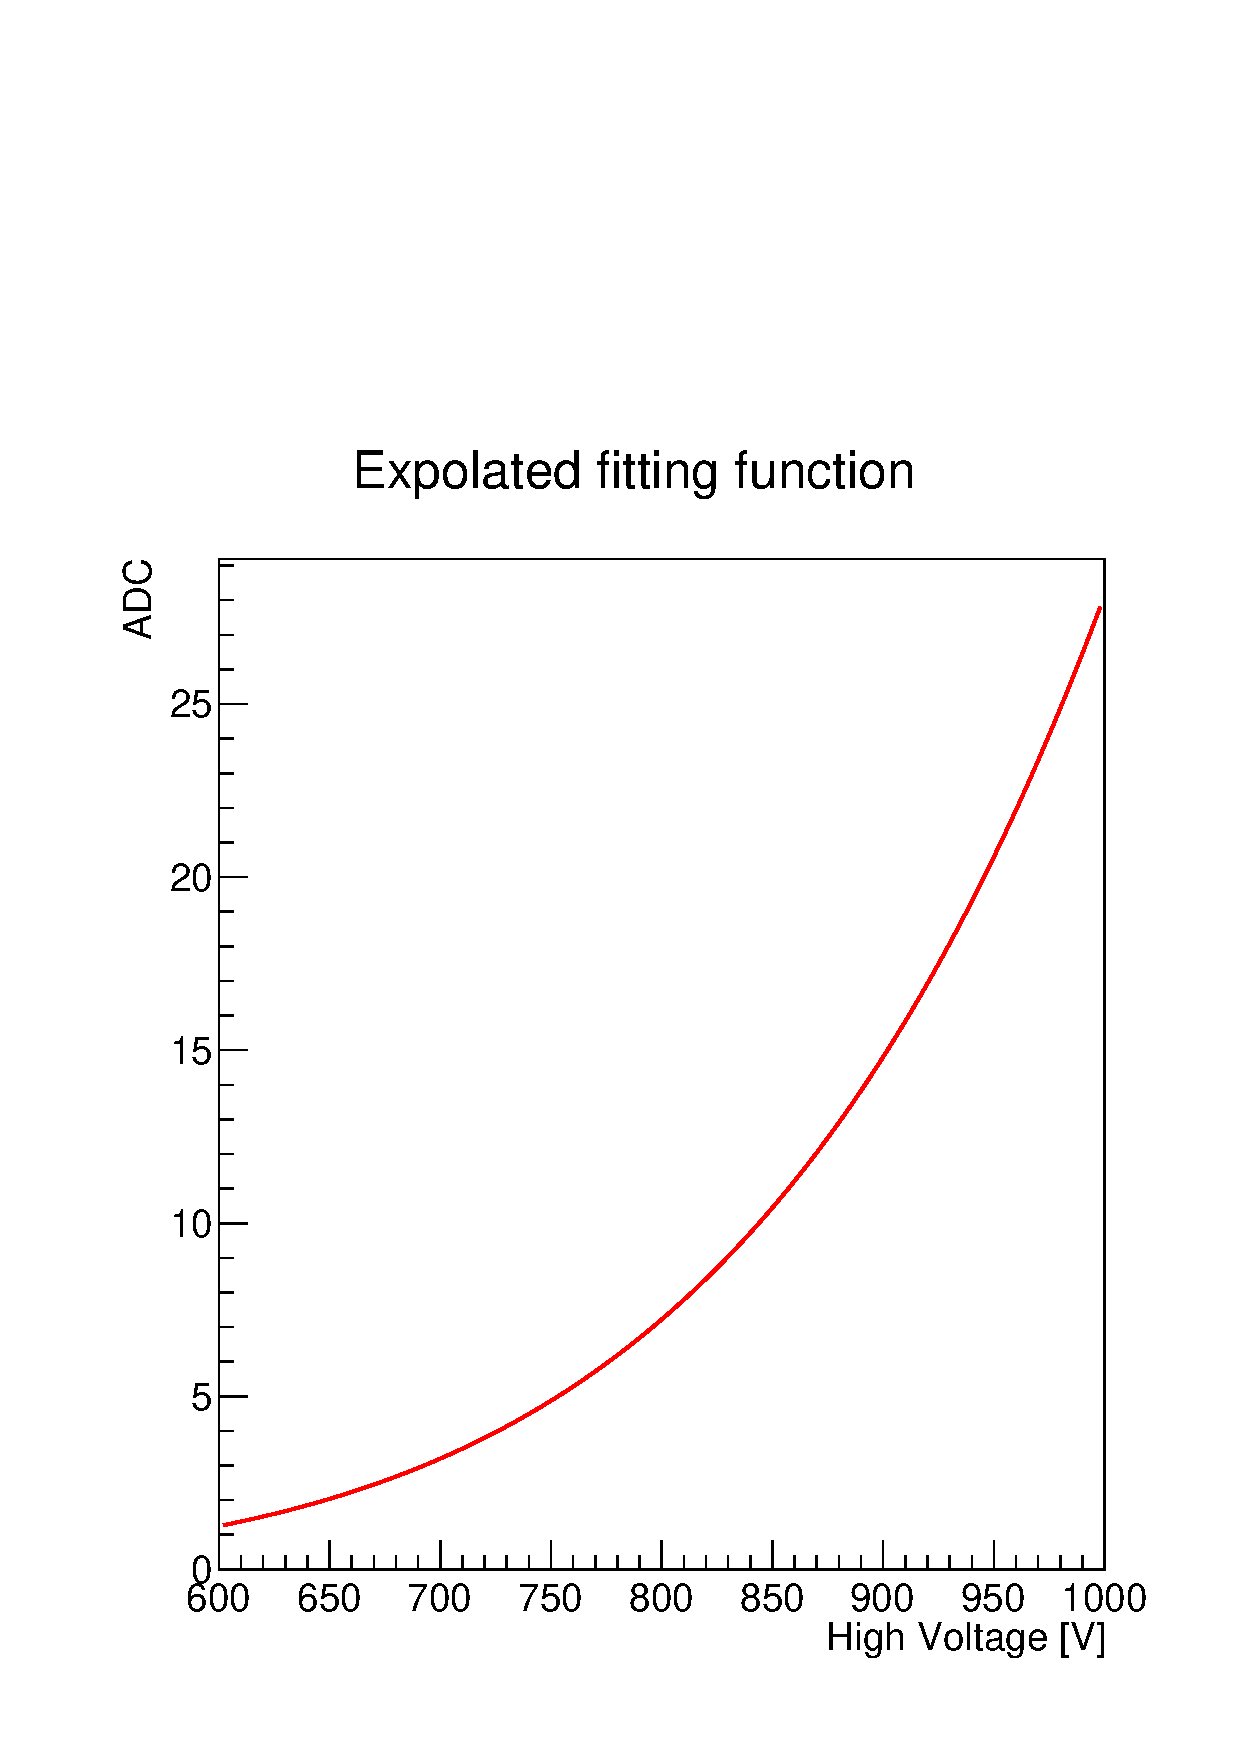
\includegraphics[width=200pt]{./Figure/EBESAnalysis/extra.pdf}
		\caption[HV scanによって得られたフィッティングの外挿曲線]{HV scanによって得られたフィッティングの外挿曲線。範囲はHVが600Vから1000Vまでに制限している。}
		\label{extra}
	\end{center}
\end{figure}

この曲線から$\SI{850}{V}$におけるADCをおよそ10.4と見積もり、今回用いたのがビームエネルギー$\SI{5.0}{GeV}$のデータであることから、HVが$\SI{850}{V}$の時のビームエネルギーとADCが図\ref{ADC_energy}のような比例関係にあるとして、バックグラウンド測定における検出器のエネルギー損失を計算した。%鉛ガラス検出器の性能評価において得られたHV scanの結果からHVが$\SI{850}{V}$の時の、鉛ガラス検出器内で生じたエネルギー損失とADCの関係を求めた。その図を\ref{ADC_energyDep}に示す。
\begin{figure}[H]
	\begin{center}
		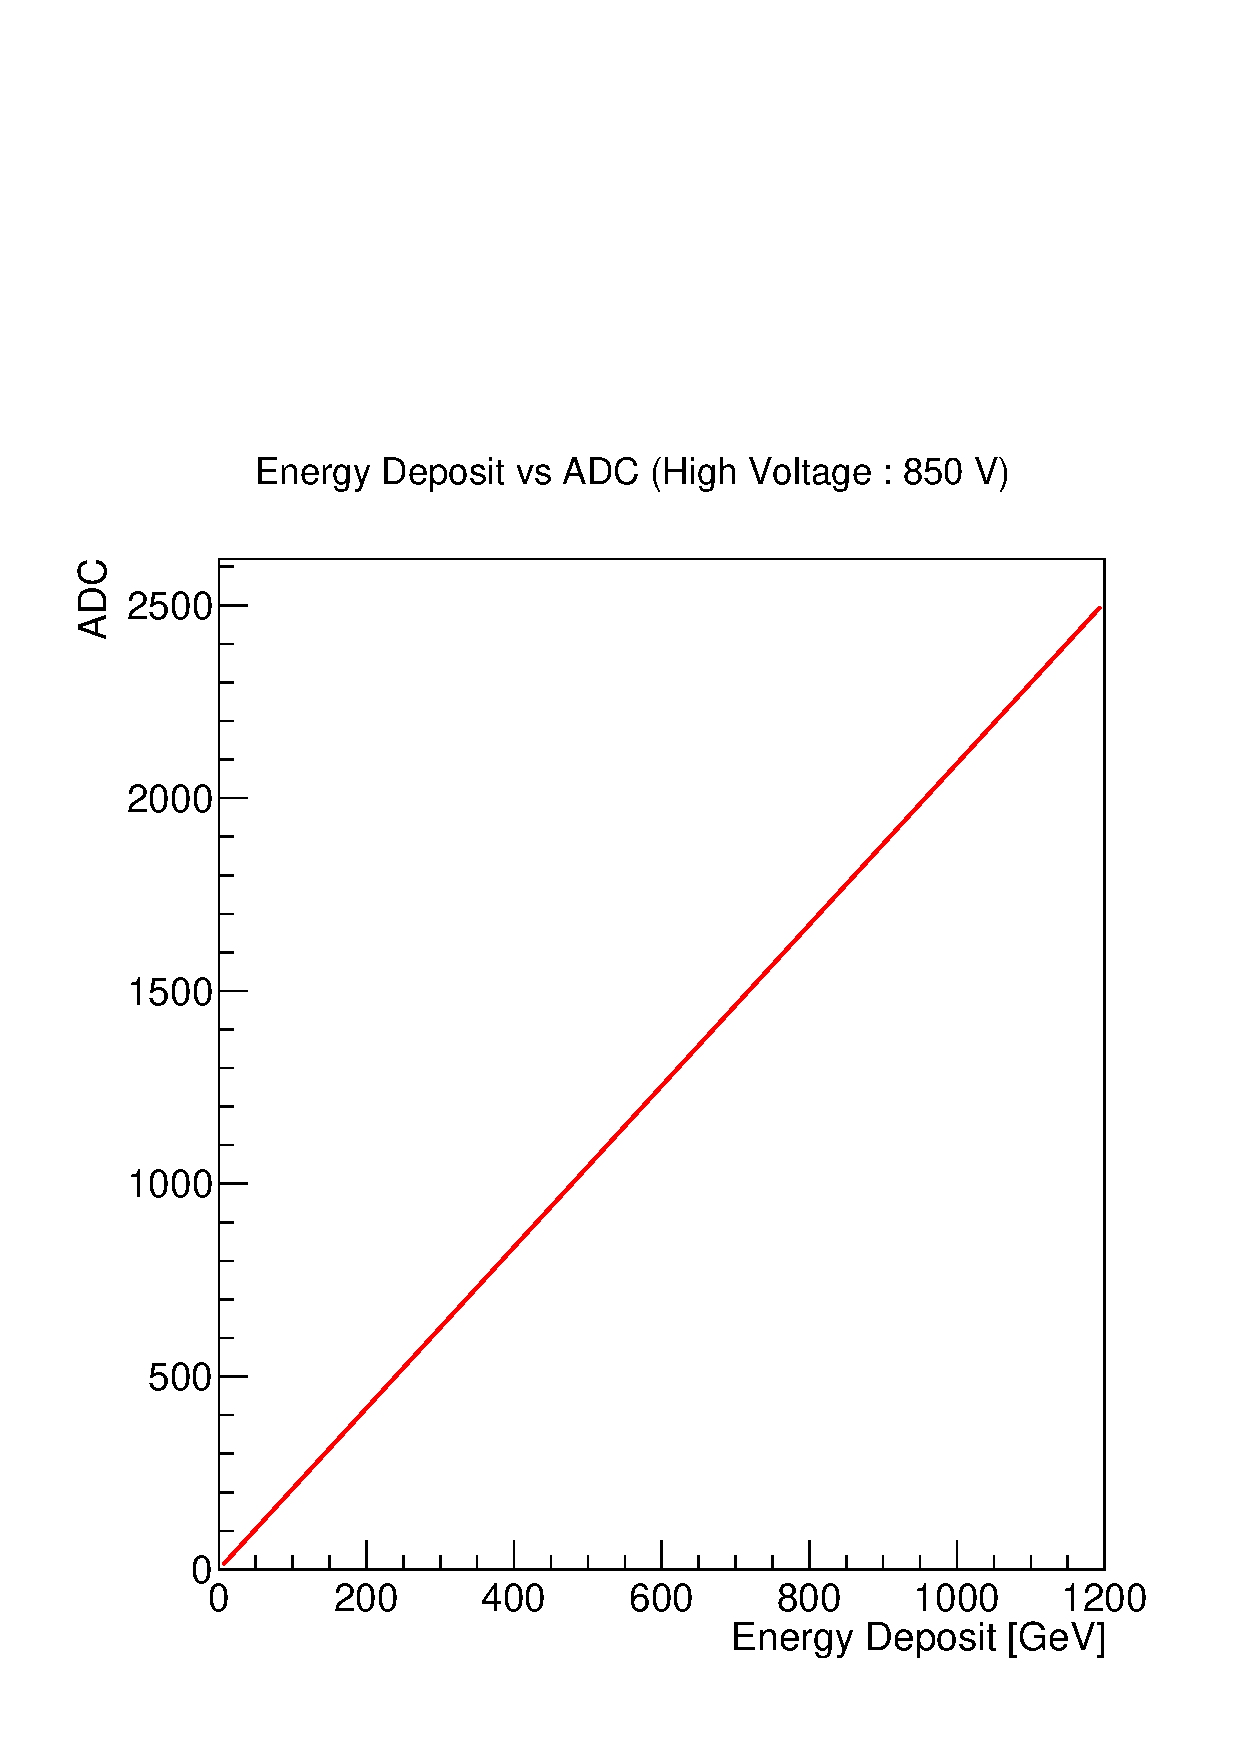
\includegraphics[width=200pt]{./Figure/EBESAnalysis/ADC_energy.pdf}
		\caption[外挿曲線から推定される$\SI{850}{GeV}$におけるビームエネルギーとADCの関係]{外挿曲線から推定される$\SI{850}{GeV}$におけるビームエネルギーとADCの関係}
		\label{ADC_energy}
	\end{center}
\end{figure}



\begin{comment}
\begin{figure}[H]
	\begin{center}
		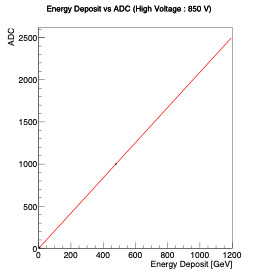
\includegraphics[width=200pt]{./Figure/EBES/ADC_energyDep.png}
		\caption[ADCと検出器内で生じたエネルギー損失の関係]{ADCと検出器内で生じたエネルギー損失の関係。}
		\label{ADC_energyDep}
	\end{center}
\end{figure}
\end{comment}
%これを用いて、一例として\ref{background_ADC}に示された検出器応答の際の入射したバックグラウンドの発生レートを計算した。
%今回は$\SI{5.0}{GeV}$におけるHVが-1400から$\SI{-1750}{V}$までのデータを用いたが、より詳細な解析のためには他のエネルギーやHV領域のデータと合わせてさらに精密な測定を行う必要がある。



